\documentclass[12pt]{article}

\usepackage{alltt}
\usepackage{epsfig}
\usepackage{pstricks}
\usepackage{xspace}
%\usepackage{makeidx}
\usepackage{index}
%\usepackage{multind}

\makeindex

\newindex{MLbn}{bnx}{bnd}{Index of ML bindings}
\newindex{MLty}{tnx}{tnd}{Index of ML types}

\newcommand{\bnind}[1]{\index[MLbn]{#1}}
\newcommand{\tyind}[1]{\index[MLty]{#1}}


\newlength{\minipagewidth}
\setlength{\minipagewidth}{\textwidth}
\addtolength{\minipagewidth}{-5mm}

\newenvironment{greekenumerate}{\begin{enumerate}
  \renewcommand{\theenumi}{\roman{enumi}}
  \renewcommand{\labelenumi}{(\roman{enumi})}}{\end{enumerate}}

\renewcommand{\t}[1]{\mbox{\tt #1}}
\newcommand{\con}[1]{\mbox{\sf #1}}
%\newcommand{\ty}[1]{\mbox{\sl #1}}
\newcommand{\ty}[1]{\mbox{\tt #1}}
\newcommand{\prev}[1]{#1}

\newcommand{\varord}[1]{#1}

\newcommand{\ma}[1]{{{$#1$}}}
\newcommand{\ml}[1]{{\tt #1}}
\newcommand{\id}[1]{#1}

\newcommand{\redonlightgray}[1]%
{\psset{fillcolor=lightgray}\psframebox*[framearc=.3]{\red #1}}

\newcommand{\termbdd}[3]{\mbox{$#1~#2~\mapsto~#3$}}
\newcommand{\globtermbdd}[2]{\mbox{$#1\hspace{0.5mm}\mapsto\hspace{0.5mm}#2$}}
\newcommand{\qq}[1]{\mbox{\tt{`\hspace{-1.3mm}`}}#1\mbox{\tt{`\hspace{-1.3mm}`}}}

\newcommand\termbddty{\ty{term\_bdd}}

\newcommand\HOL{HOL\xspace}
\newcommand\Hol{Hol98\xspace}
\newcommand{\mosml}{Moscow~ML\xspace}
\newcommand{\Buddy}{BuDDy\xspace}
\newcommand{\Muddy}{MuDDy\xspace}
\newcommand\HolBuddy{{Hol98{+}\Buddy\xspace}}

%\newcommand\fun{{\to}}
\newcommand\fun{\mbox{\tt{->}}}
\newcommand\turn{{\vdash}}
\newcommand\imp{{\Rightarrow}}
\newcommand\T{\con{T}}
\newcommand\F{\con{F}}

\newcommand{\cond}{\rightarrow}
\newcommand{\els}{\mid}
\newcommand{\Imp}{\Rightarrow}

%\renewcommand{\prod}{\times}
\renewcommand{\prod}{\mbox{\tt{*}}}
\newcommand{\SP}{~}
\newcommand{\SPP}{~}

\newcommand{\homedir}{\mbox{$\sim$}}

\newcommand{\Turn}{\(\turn\)}
\newcommand{\And}{\(\wedge\)}
\newcommand{\Or}{\(\vee\)}
\newcommand{\Not}{\(\neg\)}
\newcommand{\Forall}{\(\forall\)}
\newcommand{\Exists}{\(\exists\)}
\newcommand{\Mapsto}{\(\mapsto\)}


\parindent 0mm
\parskip 1mm


% ---------------------------------------------------------------------
% Macros for little HOL sessions displayed in boxes.
%
% Usage: (1) \setcounter{sessioncount}{1} resets the session counter
%
%	 (2) \begin{session}\begin{verbatim}
%	      .
%	       < lines from hol session >
%	      .
%	     \end{verbatim}\end{session}   
%
%            typesets the session in a numbered box.
% ---------------------------------------------------------------------

\newlength{\hsbw}
\setlength{\hsbw}{\textwidth}
\addtolength{\hsbw}{-\arrayrulewidth}
\addtolength{\hsbw}{-\tabcolsep}

\newcounter{sessioncount}
\setcounter{sessioncount}{1}

\newcommand\MLSpacing{13pt}
\newenvironment{session}{\begin{flushleft}
 \begin{tabular}{@{}|c@{}|@{}}\hline 
 \begin{minipage}[b]{\hsbw}
 \vspace*{-.5pt}
 \begin{flushright}
 \rule{0.01in}{.15in}\rule{0.3in}{0.01in}\hspace{-0.35in}
 \raisebox{0.04in}{\makebox[0.3in][c]{\footnotesize\sl \thesessioncount}}
 \end{flushright}
 \vspace*{-.45in}
 \begingroup\small\baselineskip\MLSpacing}{\endgroup\end{minipage}\\ \hline 
 \end{tabular}
 \end{flushleft}
 \stepcounter{sessioncount}}

\begin{document}
\thispagestyle{empty}

\hrule height5pt

\begin{flushleft}\Huge
{\tt HolBddLib} Documentation
\end{flushleft}

\vspace*{2mm}

\hrule height5pt

\vspace*{1cm}


\noindent{\Large{\bf Mike Gordon}}

\vspace*{5mm}

\today

\vfill

{\setlength{\fboxrule}{0.5mm}
\setlength{\fboxsep}{2mm}
\fbox{
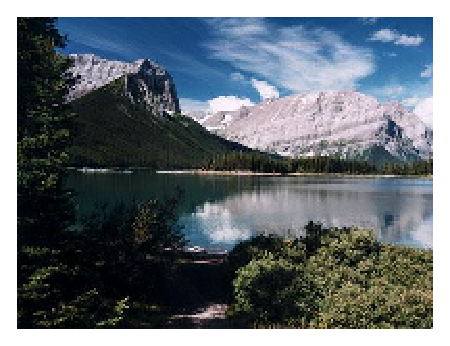
\epsfig{file=kananaskis_small.ps} \raisebox{2.5cm}{\Huge\bf~~~+~} 
\raisebox{0mm}{\epsfig{file=scratchBDD.ps, height=5.3cm, width=3.5cm}}
}}

\vfill

\newpage

\pagenumbering{roman}

\section*{Preface}



This document describes {\tt{HolBddLib}}
as distributed with the {\it Kananaskis\/} release of Hol98.

{\tt{HolBddLib}} provides infrastructure in Hol98 for building 
`fully-expansive' or `LCF-style' symbolic calculation algorithms, like model
checkers, that use binary decision diagrams (BDDs). 

The development of {\tt HolBddLib} has gone through two phases so far
(more are expected) and consists of tools
from the second phase implemented on top of code resulting from
experiments dating from the first phase.  This evolution is described in
general terms in Part~\ref{overview}, which is an updated version of a
paper presented at the 13th International Conference on Theorem
Proving and Higher Order Logics (TPHOLs2000) \cite{Gordon:TPHOLs2000}.

{\tt HolBddLib} uses J{\o}rn Lind-Nielsen's \Buddy{} package as a BDD
engine. The interface from \Buddy{} to Moscow ML, called \Muddy, is
due to Ken Friis Larsen and is described in Part~\ref{muddy}.

{\tt HolBddLib} is built on top of \Muddy{} and
is described in Part~\ref{HolBddLib}.
The first phase of development of {\tt HolBddLib} resulted in the
modules {\tt HolBdd} and {\tt StateEnum} and the second phase resulted
in module {\tt BddRules}.

Some of the material in Part~\ref{muddy} and Part~\ref{HolBddLib} 
is based on the University of Cambridge Computer Laboratory Technical
Report No.~481, December 1999, by Mike Gordon and Ken Friis Larsen
\cite{GordonLarsen}. This report has examples that might be of
tutorial use, however they reflect the first phase of the development
of {\tt HolBddLib} and contain some obsolete methodology, so have been
omitted from this document.

\vfill

\begin{flushright}
Mike Gordon\\
\today
\end{flushright}


\newpage

{\baselineskip10pt
\tableofcontents
}

\newpage
                     
\part{Reachability programming in \Hol{} using BDDs}\label{overview}

\pagenumbering{arabic}

\begin{quote}\it
This part is a revised and corrected version of a paper presented at the 13th International
Conference on Theorem Proving and Higher Order Logics (TPHOLs2000)
\cite{Gordon:TPHOLs2000}. The revisions consist in making
the descriptions match the current release of \ml{HolBddLib}.
Some of these descriptions need to be read in conjunction with
the documentation of \Muddy{} in Part~\ref{muddy} (forward pointers have been added).
\end{quote}

\section{Abstract}
Two methods of programming BDD-based symbolic algorithms in the Hol98
proof assistant are presented. The goal is to provide a platform for
implementing intimate combinations of deduction and algorithmic
verification, like model checking.  The first programming method uses
a small kernel of ML functions to convert between BDDs, terms and
theorems. It is easy to use and is suitable for rapid prototying
experiments.  The second method requires lower-level programming but
can support more efficient calculations. It is based on an LCF-like
use of an abstract type to encapsulate rules for manipulating
judgements $\termbdd{\rho}{t}{b}$ meaning ``logical term $t$ is
represented by BDD $b$ with respect to variable order $\rho$''.  The
two methods are illustrated by showing how to perform the standard
fixed-point calculation of the BDD of the set of reachable states of a
finite state machine.

\section{Background and motivation}

Theorem proving and model checking are complementary. Theorem proving
can be applied to expressive formalisms (such as set theory and higher
order logic) that are capable of modelling complex systems like
complete processors. However, theorem proving systems require skilled
manual guidance to verify most properties of practical interest. Model
checking is automatic, but can only be applied to relatively small
problems (e.g.~fragments of processors). It can also provide
counter-examples of great use in debugging.

The ideal would be to be able to automatically verify properties of
complete systems (and find counter-examples when the verification of
properties fail).  This is not likely to be practical in the
foreseeable future, so various compromises are being explored, for
example

\begin{greekenumerate}
\item adding a layer of theorem proving on top of existing model
checkers, to enable large problems to be deductively decomposed into
smaller pieces that can be checked automatically 
\cite{McMillan99,aagaard-tphols-99};

\item adding checking algorithms to theorem provers so that subgoals
can be verified automatically \cite{Rajan95:CAV} and counter-examples found.
\end{greekenumerate}

These two approaches differ in the starting point: (i) starts from a
model checker and (ii) starts from a theorem prover. The goal is the same: 
combine the best of model checking and theorem proving. This paper concerns approach (ii).

The Prosper
project\footnote{\tt{http://www.dcs.gla.ac.uk/prosper}}  is
currently undertaking research into making \HOL{} the basis of a tool
integration platform. Part of this work has resulted in the definition
and implementation of a mechanism for enabling external tools to
be `plugged-in' to \HOL.  This supports the easy implementation of the
kind of linking of theorem proving and model checking done in
pioneering studies with PVS \cite{Rajan95:CAV} and falls under (ii) above.

This paper describes some experiments in adding simple model checking
infrastructure to the \Hol{} theorem prover and so also falls under
(ii).  However, it differs from the PVS and Prosper approaches because
it aims to provide secure and general programming infrastructure to
allow users to implement {\em their own} bespoke BDD-based
verification algorithms and then to tightly integrate them with
existing \HOL{} tools like the simplifier. Sometimes it is appropriate
to use an existing off-the-shelf tool and sometimes it is appropriate
to build one's own bespoke solution. This paper concerns the latter.

The \HOL{} system is based on Milner's LCF proof assistant
\cite{EdinLCF}.  In such systems arbitrary terms are values of a type
\ty{term}\tyind{\ml{term}} and can be freely constructed. However, theorems are
represented as values of an abstract type \ty{thm}\tyind{\ml{thm}} whose primitive
operations are axioms and rules of inference.  Being an abstract type,
values of type \ty{thm} (i.e.~theorems) can only by constructed using
combinations of the primitive operations provided for the type
\ty{thm} -- i.e.~by proof.  Theorem proving tools such as decision
procedures, proof search strategies and simplifiers are implemented by
composing together the primitive operations (i.e.~axioms and inference
rules) using programs in the ML programming language.

The goal of the research described in this paper is to extend the
classical LCF-approach so that efficient symbolic calculations, like
model checking, can also be implemented. This involves generalising
the notion of theorem to include certain data representation
judgements.






\section{Overview}

Let ${\cal M}$ be a finite state machine whose state is a vector
$(v_1,\ldots,v_n)$ of boolean variables
$v_1,\ldots,v_n$.
Let
\con{P} be some property of interest  of states of  ${\cal M}$ and
let $\con{S}$ be defined so that
$\con{S}~i~(v_1,\ldots,v_n)$ is true if $(v_1,\ldots,v_n)$ is a state
reachable in $i$ or fewer steps from an initial state of ${\cal M}$.

Any boolean term with boolean free variables
can be represented by a binary
decision diagram (BDD) \cite{BryantSurvey}. An example of such a term is:

\smallskip

~$\forall i.~\con{S}~i~(v_1,\ldots,v_n)~\imp~\con{P}(v_1,\ldots,v_n)$

\smallskip

This is true if all
reachable states of ${\cal M}$ satisfy \con{P}. Note that although this
term and all its free variables are boolean, it contains a bound
variable $i$ ranging over natural numbers, so the standard BDD
algorithms cannot construct its BDD. However, 
symbolic model checking algorithms provide ways of computing the BDDs
of such terms. These algorithms can also
compute the BDDs corresponding to much more complex properties of the
execution of finite state machines (e.g.~properties expressed in
temporal logic).

In order to provide a platform for experimenting with programming
model checking algorithms in the \Hol{} proof assistant, and for
combining them with deductive theorem proving, the \Buddy{}
package\footnote{\texttt{http://www.itu.dk/research/buddy/}} has been
interfaced\footnote{\texttt{http://www.itu.dk/research/muddy/}} to Moscow 
ML\footnote{\texttt{http://www.dina.kvl.dk/{\homedir}sestoft/mosml.html}}
so that BDDs can be manipulated as ML values of a type \ty{bdd}\tyind{\ml{bdd}}
and the various \Buddy{} operations are linked to ML functions.
%The \Hol{} library \texttt{HolBddLib}  uses the Moscow ML interface to ML
%to prove BDD tools for \Hol{} \cite{GordonLarsen}.

In this paper, the evolution of an initial simple style of programming
with BDDs into a more efficient one is described.  
The computation of
the set of reachable states is used as a running example
(more detailed examples are described elsewhere \cite{mjcg99a,GordonLarsen}).  
Note that

\smallskip

~$\forall i.~\con{S}~i~(v_1,\ldots,v_n)~\imp~\con{P}(v_1,\ldots,v_n)$

\smallskip

\noindent is equivalent to


\smallskip

~${\mbox{\large$($}}\exists i.~\con{S}~i~(v_1,\ldots,v_n){\mbox{\large$)$}}~\imp~\con{P}(v_1,\ldots,v_n)$

\smallskip
\noindent The set of reachable states is
represented by the term $\exists i.~ \con{S}~i~(v_1,\ldots,v_n)$.

The first method is described in Section~\ref{method1} and is based
on a validity-critical kernel of three
ML functions:


\smallskip

$\begin{array}{ll}\bnind{\ml{termToBdd}}\bnind{\ml{addEquation}}\bnind{\ml{bddOracle}}
\ml{termToBdd}   &: \ty{term}~\fun~\ty{bdd}\\
\ml{addEquation} &: \ty{thm}~\fun~\ty{term}\prod\ty{bdd}\\
\ml{bddOracle}   &: \ty{term}~\fun~\ty{thm}\\
\end{array}$

\smallskip

As long as these are implemented correctly (which includes
\Buddy{} being correct) then the system is sound.
The use of these functions to compute the BDD of $\exists i.~ \con{S}~i~(v_1,\ldots,v_n)$
is described in Section~\ref{reach1}.

The second method uses an abstract type $\termbddty$\tyind{\ml{term\_bdd}} that represents
`judgements' $\termbdd{\rho}{t}{b}$ that mean ``\Hol{} term $t$ is
represented by BDD $b$ with respect to variable order $\rho$''.  An
LCF-like approach to `proving' such judgements is implemented: the
type $\termbddty$ implements judgements just like the type $\ty{thm}$
implements theorems.  A fragment of the calculus of BDD representation
judgements is presented in Section~\ref{judgements} (with some planned
extensions in Section~\ref{future}). The ML functions implementing
rules of inference for judgements are given in boxes following the
rules. The calculation of $\exists i.~ \con{S}~i~(v_1,\ldots,v_n)$
using judgements is described in Section~\ref{reach2}.

Some related work is discussed in Section~\ref{related}.

\section{Representing terms as BDDs}\label{method1}

The interface from \Buddy{} to \mosml{} provides an ML type \ty{bdd}\tyind{\ml{bdd}} together with
ML functions corresponding to the C functions in the BDD
package.
Using these, it is easy to implement a function that maps any quantified
boolean formula\footnote{A quantified boolean formula (QBF) is a term
build out of boolean variables and constants (\con{T}, \con{F}) using
boolean operators ($\neg$, $\wedge$, $\vee$, $\imp$, $=$ etc.) and
quantification over boolean variables.} to a
BDD. Such a function has ML type $\ty{term}\fun\ty{bdd}$ and is
defined by a simple recursion over the structure of
terms.\footnote{The recursion needs to take into account BDD
operations that optimise certain combinations of boolean
constructions. For example, the BDD of a term $\con{Q}v_1\cdots
v_n.~t_1~\con{op}~t_2$, where \con{Q} is a quantifier and \con{op} a
binary operator, can be efficiently constructed from the BDDs of $t_1$
and $t_2$ in a single step. First constructing the BDD of
$t_1~\con{op}~t_2$ and then doing $n$ quantifications would be
inefficient.}

Two approaches to supporting BDD calculation in \Hol{} are described
here. The first one is described in this section and is based on a global
table that stores pairs $(t,b)$, where $t$ is a term and $b$ the BDD
representing it. The second approach is described in
Section~\ref{second}. 
%If $b$ is the BDD representing $t$, then the
%pair $(t,b)$ will be written $t\mapsto b$. 
%For example, at the third
%stage of an iteration to compute the BDD of the set of reachable
%states of machine ${\cal M}$, the table might consist of the entries
%$(\con{S}~0~(v_1,\ldots,v_n),~b_0)$,
%$(\con{S}~1~(v_1,\ldots,v_n),~b_1)$ and
%$(\con{S}~2~(v_1,\ldots,v_n),~b_2)$.

The \Hol{} library \texttt{HolBddLib}  uses the Moscow ML interface to ML
to implement BDD tools for \Hol{} \cite{GordonLarsen}.
This library predefines the following ML function for adding
entries to the BDD table

\smallskip

$~\ml{addEquation} : \ty{thm}~\fun~\ty{term}\prod\ty{bdd}$\bnind{\ml{addEquation}}

\smallskip

\noindent Evaluating $\ml{addEquation}(\vdash t_1 = t_2)$ computes a
BDD, $b_2$ say, of the term $t_2$ and then stores the association
$(t_1,b_2)$ in the BDD table. The pair $(t_1,b_2)$ is also
returned.\footnote{An exception is raised by \ml{addEquation} if it is
not applied to an equation or if the computation of the BDD of $t_2$
fails.}

Using the BDD table, the BDDs of boolean terms that contain defined constants
can be computed. For example, suppose the constant \con{Foo} is defined by

\smallskip

~$\vdash \con{Foo}(x,y) = \langle\mbox{\it{large QBF involving x and y}}\rangle$

\smallskip

\noindent then the BDDs of terms such as 
$\exists z.~\con{Foo}(x,(y~\vee~z))~\wedge~\con{Foo}(z,(x~\imp~y))$
can be computed in two ways:
(i) by expanding out the definition of \con{Foo} to get a QBF;
and (ii) by using the precomputed BDD of $\con{Foo}(x,y)$ stored in the table.

The choice between (i) and (ii) depends on whether
it is more efficient to separately recompute the BDDs of $\con{Foo}(x,(y~\vee~z))$
and $\con{Foo}(z,(x~\imp~y))$ from scratch or to get the BDDs by
applying \Buddy{} operations to the BDD of $\con{Foo}(x,y)$. 

An ML function \ml{termToBdd}\bnind{\ml{termToBdd}} of type $\ty{term}\fun\ty{bdd}$ is
provided by \ml{HolBddLib} that uses the second method (ii) to convert
a term to a BDD.  This works by deductively transforming terms to a
form in which subterms correspond to entries in the BDD table.  

For
example, applying \ml{termToBdd} to $\exists
z.~\con{Foo}(x,(y~\vee~z))~\wedge~\con{Foo}(z,(x~\imp~y))$
% ?z. Foo(x,(y \/ z)) /\ Foo(z,(x ==> y))
first uses a \Hol{} conversion to prove the theorem

\smallskip
$\begin{array}{l}
\vdash (\exists z.~ \con{Foo}(x,(y~\vee~z))~\wedge~\con{Foo}(z,(x~\imp~y))\\
\phantom{\vdash} 
=\\
\phantom{\vdash}
 (\exists z.~(\exists y_1.~ (y_1 = y \vee z) \wedge \con{Foo}(x,y_1))
~\wedge~
\exists y_1.~(y_1 = x \imp y) ~\wedge \con{Foo}(z,y_1))
\end{array}$

\smallskip

\noindent The BDD of the left hand side of this equation can then be
computed by computing the BDD of the right hand side, in which all
applications of \con{Foo} have been transformed to be applied to sequences of
distinct variables. The BDD of such applications can be obtained by a
simple replacement operation on the BDD of $\con{Foo}(x,y)$ and so the
BDD of the large term on the right hand side of the definition of
\con{Foo} does not need to be recomputed, just tweaked.

The BDD representing a term is determined by an ordering of the
variables.  The variable order used by \ml{termToBdd} can be
explicitly declared, but if no order is declared, then variables get the
order in which they are first encountered.

The creation of \Hol{} theorems via BDD calculation is provided
by a single ML function
$\ml{bddOracle} : \ty{term}~\fun~\ty{thm}$\bnind{\ml{bddOracle}}
which maps a term $t$ to the theorem $\vdash t$ if
\ml{termToBdd(}$t$\ml{)} is the BDD \ml{TRUE} and raises
an exception otherwise.

%Thus, in summary, the first approach to linking BuDDy and \Hol{} consists of 
%a validity-critical kernel of three
%ML functions:
%
%
%\smallskip
%
%~$\begin{array}{ll}
%\ml{termToBdd}   &: \ty{term}~\fun~\ty{bdd}\\
%\ml{addEquation} &: \ty{thm}~\fun~\ty{term}\prod\ty{bdd}\\
%\ml{bddOracle}   &: \ty{term}~\fun~\ty{thm}\\
%\end{array}$
%
%\smallskip
%
%As long as these are implemented correctly (which includes
%BuDDy being correct) then false theorems cannot be proved.

\subsection{Computing reachable states using first method}\label{reach1}

Suppose constants \con{B} and \con{R} are defined to represent,
respectively, a set of initial states of a machine and its transition
relation:

\smallskip

$\begin{array}{l}
\ml{B\_def}~=~\vdash \con{B}(v_1,\ldots,v_n)~=~\cdots\\
\ml{R\_def}~=~\vdash \con{R}((v_1,\ldots,v_n),(v'_1,\ldots,v'_n))~=~\cdots\\
\end{array}$

\smallskip
The predicate $\con{S}~i$ repesenting the set of states reachable in
$i$ or fewer steps is then defined recursively by

\smallskip

$\begin{array}{l}
\ml{S\_def}~=~\vdash (\con{S}~0~v~=~\con{B}~v)\\
\phantom{\ml{S\_def}~=~\vdash }
 ~\wedge\\
\phantom{\ml{S\_def}~=~\vdash }
~\forall i.~\con{S}~(i{+}1)~v~ =~(\con{S}~i~v~\vee~(\exists u.~\con{S}~i~u~\wedge~\con{R}(u,v)))\\
\end{array}$

\smallskip

\noindent where the variables $u$ and $v$ range over $n$-tuples of booleans and
so can be specialised to tuples of boolean variables $(u_1,\ldots,u_n)$ and
$(v_1,\ldots,v_n)$, respectively, and then separate
base and step cases derived as theorems \ml{S\_0} and \ml{S\_suc}, where

\smallskip

$\begin{array}{ll}
\ml{S\_0}~&=~\vdash \con{S}~0~(v_1,\ldots,v_n)~=~\con{B}~(v_1,\ldots,v_n)\\

\ml{S\_suc}~&=~\vdash \forall i.~\con{S}~(i{+}1)~(v_1,\ldots,v_n)~ =\\
& \phantom{=~\vdash \forall i.~~}
\con{S}~i~(v_1,\ldots,v_n)\\
& \phantom{=~\vdash \forall i.~~}
\vee\\
& \phantom{=~\vdash \forall i.~~}
\exists u_1~\cdots~u_n.~\con{S}~i~(u_1,\ldots,u_n)~\wedge~\con{R}((u_1,\ldots,u_n),(v_1,\ldots,v_n))
\end{array}$

\smallskip


To compute the
BDD of the set of reachable states, first add the definitions of \con{B} and \con{R}
to the BDD table:


\smallskip

$\begin{array}{ll}
\ml{addEquation~B\_def};\\
\ml{addEquation~R\_def};
\end{array}$

\smallskip

\noindent next compute the BDDs of
$\con{S}~0~(v_1,\ldots,v_n)$,  $\con{S}~1~(v_1,\ldots,v_n)$, $\con{S}~2~(v_1,\ldots,v_n)$ etc.
Note from \ml{S\_suc} that the compution of of the BDD of $\con{S}~(i{+}1)~(v_1,\ldots,v_n)$
needs the BDD of $\con{S}~i~(v_1,\ldots,v_n)$, thus the order in which BDDs are added to the
table is important. The $\forall$-quantified variable $i$ in \ml{S\_suc} can be successively
specialised to $0$, $1$, $2$ etc.~with
the \HOL{} inference rule \ml{SPEC} (evaluating
\ml{SPEC~$t_1$~(\hspace{0.5mm}$\vdash \forall i.~t_2(i)$)} specialises $i$
to $t_1$ to deduce
$\vdash t_2(t_1)$). To then reduce the numeral $\con{i}{+}1$, the function
\ml{SimpNum} can be  used (\ml{SimpNum} reduces arithmetical combinations of
numerals, e.g.~simplifies \ml{\qq{2+1}} to \ml{\qq{3}},
it can be defined by:
{\verb+val SimpNum = CONV_RULE(reduceLib.REDUCE_CONV)+}).


\smallskip

$\begin{array}{ll}
\ml{addEquation~S\_0};\\
\ml{addEquation~(SimpNum(SPEC \qq{0} S\_suc))};\\
\ml{addEquation~(SimpNum(SPEC \qq{1} S\_suc))};\\
\ml{addEquation~(SimpNum(SPEC \qq{2} S\_suc))};\\
\end{array}$

\smallskip

\noindent After these
six applications of \ml{addEquation}, the BDD table will consist of

\smallskip

$\begin{array}{l}
(\con{B}(v_1,...,v_n),~b_1)\\
(\con{R}((v_1,...,v_n),(v'_1,...,v'_n)),~b_2)\\
(\con{S}~0~(v_1,...,v_n),~b_3)\\
(\con{S}~1~(v_1,...,v_n),~b_4)\\
(\con{S}~2~(v_1,...,v_n),~b_5)\\
(\con{S}~3~(v_1,...,v_n),~b_6)
\end{array}$

\smallskip

\noindent where, in fact, $b_1=b_3$. Note that an evaluation of  


\smallskip

$\begin{array}{l}
\ml{addEquation~(SimpNum(SPEC \qq{\con{i}} S\_suc))};\\
\end{array}$

\smallskip

\noindent uses \ml{termToBdd} to compute the BDD of the 
right hand side of \ml{S\_suc} with $i$ specialised to $\con{i}$. Since the BDDs of 
$\con{S}~\con{i}~(v_1,...,v_n)$ and 
$\con{R}((v_1,...,v_n),(v'_1,...,v'_n))$ are already in the BDD table
their BDDs can be reused.

Since the state space is finite and the sets of states represented
by $\con{S}~i$ increases as $i$ increases, it follows that for some particular
$i$, say $i=\con{i}$, that
eventually 

\smallskip

~$\con{S}~i~(v_1,...,v_n)~=~\con{S}~(i{+}1)~(v_1,...,v_n)$

\smallskip

\noindent which can be tested for at each stage by evaluating:

\smallskip

~\ml{bddOracle $\qq{\con{S}~i~(v_1,...,v_n)~=~\con{S}~(i{+}1)~(v_1,...,v_n)}$}

\smallskip

This will either raise an exception (fixed-point not yet
reached) or return a theorem
$\vdash \con{S}~\con{i}~(v_1,...,v_n)~=~\con{S}~(\con{i}{+}1)~(v_1,...,v_n)$.
When this theorem is proved, the BDD of the set of reachable states
is clearly the BDD of $\con{S}~\con{i}~(v_1,...,v_n)$ (see the theorem \ml{FpTh} below).

The fixed-point is easily computed by an ML function that
makes use of the
auxiliary functions described in the following table.


\smallskip
~\begin{tabular}{|l|l|l|} \hline
~ML function       ~&~ ML type                  ~&~  Explanation \\ \hline\hline
~\ml{intToTerm}\bnind{\ml{intToTerm}}    ~&~ $\ty{int}\fun\ty{term}$  ~&~ \ml{intToTerm~n~=~\qq{n}}\\ \hline
~\ml{concl}\bnind{\ml{concl}}        ~&~ $\ty{thm}\fun\ty{term}$  ~&~ \ml{concl}($\vdash t$)~=~ \ml{\qq{$t$}}\\ \hline
~\ml{lhs}\bnind{\ml{lhs}}          ~&~ $\ty{term}\fun\ty{term}$ ~&~ \ml{lhs \qq{$t_1$=$t_2$}~=~\qq{$t_1$}}\\  \hline
~\ml{rhs}\bnind{\ml{rhs}}          ~&~ $\ty{term}\fun\ty{term}$ ~&~ \ml{rhs \qq{$t_1$=$t_2$}~=~\qq{$t_2$}}\\  \hline
~\ml{LeftDisjunct}\bnind{\ml{LeftDisjunct}} ~&~ $\ty{term}\fun\ty{term}$ ~&~ \ml{LeftDisjunct \qq{$t_1 \vee t_2$}~=~\qq{$t_1$}}~~\\  \hline
~\ml{mk\_eq}       ~&~ $\ty{term}{\prod}\ty{term}\fun\ty{term}$ ~&~ \ml{mk\_eq(\qq{$t_1$},\qq{$t_2$})~=~\qq{$t_1$=$t_2$}}\\  \hline
\end{tabular}
\smallskip

\noindent In the function definitions below, 
ML comments are enclosed between \ml{(*} and \ml{*)}.

\vspace*{-1mm}

\begin{verbatim}
 fun LeftDisjunct tm = fst(Psyntax.dest_disj tm);

 fun iterateToFixedPoint S_suc i =
  let val i_tm = intToTerm i
      val Sth  = SimpNum(SPEC i_tm S_suc)
      val S1   = LeftDisjunct(rhs(concl Sth)) (* S i (...)     *)
      val S2   = lhs(concl Sth)               (* S (i+1) (...) *)
  in
   addEquation Sth;  (* adds BDD of S (i+1) (...) to BDD table *)
   (bddOracle(mk_eq(S1,S2)), i_tm)
    handle oracleError => iterateToFixedPoint S_suc (i+1)
  end
\end{verbatim}\bnind{\ml{iterateToFixedPoint}}

\vspace*{-1mm}

The function \ml{iterateToFixedPoint} just iterates \ml{S\_suc} until
a fixed-point is reached and then, if the fixed-point is reached after
\con{i} iterations, returns a pair whose second component is $\qq{\con{i}}$ and 
whose first component is the theorem:

\smallskip

~$\vdash \con{S}~\con{i}~(v_1,...,v_n)~=~\con{S}~(\con{i}{+}1)~(v_1,...,v_n)$

\smallskip

\noindent The following fixed-point theorem
is straightforward to prove


\smallskip

$\begin{array}{ll}
\ml{FpTh}~=~\vdash \forall i.~& (\forall v_1\cdots v_n.~\con{S}~i~(v_1,...,v_n)~=~\con{S}~(i{+}1)~(v_1,...,v_n))\\
 &\imp\\
& (\forall v_1\cdots v_n.~\con{S}~i~(v_1,...,v_n)~=~\exists i.~\con{S}~i~(v_1,...,v_n))
\end{array}$

\smallskip

\noindent The function \ml{ComputeReachableStates}\bnind{\ml{ComputeReachableStates}} defined below
computes a pair, returned by \ml{addEquation}, whose first component is the term
$\exists i.~\con{S}~i~(v_1,...,v_n)$ and whose second component is the BDD of this term.
The definition of the function uses 
Modus Ponens, which is represented by the ML function \ml{MP}
(evaluating
$\ml{MP}~(\vdash t_1\imp t_2)~(\vdash t_1)$ 
returns the theorem $\vdash t_2$). The definition also uses
\ml{GEN\_ALL}, which
proves the universal closure of a theorem (i.e.~universally quantifies all free variables),
and \ml{SYM}, which  reverses an equation (evaluating $\ml{SYM}(\vdash t_1=t_2)$
returns the theorem $\vdash t_2=t_1$).

\vspace*{-1mm}

\begin{verbatim}
 fun ComputeReachableStates B_def R_def S_0 S_suc =
  (addEquation B_def;
   addEquation R_def;
   addEquation S_0;
   let val (th,i_tm) = iterateToFixedPoint S_suc 0
   in
    addEquation(SYM(MP (SPEC i_tm FpTh) (GEN_ALL th)))
   end)
\end{verbatim}

\vspace*{-1mm}

The theorems \ml{S\_0} and \ml{S\_suc} are just consequences
of the definition of \con{S}, so could be computed from
\ml{B\_def} and \ml{R\_def}. Thus \ml{ComputeReachableStates}
only needs to take \ml{B\_def} and \ml{R\_def} as parameters
\cite{mjcg99a}.

Note that executing {\verb+ComputeReachableStates B_def R_def S_0 S_suc+}
involves computing the BDD of
$\con{R}((v_1,\ldots,v_n),(v'_1,\ldots,v'_n))$, which may be
large. 

Instead, it may be possible to derive an equation, \ml{S\_simp\_suc} say, that expresses
$\con{S}~(i{+}1)~(v_1,\ldots,v_n)$ in terms of
$\con{S}~i~(v_1,\ldots,v_n)$ in a way that avoids having to compute
the BDD of the transition relation. This can be achieved, for example,
by disjunctive partitioning\footnote{Disjunctive partitioning is
called `early quantification' by some authors \cite[page~45]{McMillanBook}
and also called `miniscoping' in the context of theorem proving.}
\cite[page~79]{ClarkeBook}. In this case, the calculation of reachable states can be done just with

\vspace*{-1mm}

\begin{verbatim}
 fun ComputeReachableStates B_def R_def S_0 S_simp_suc =
  (addEquation B_def;
   addEquation S_0;
   let val (th,i_tm) = iterateToFixedPoint S_simp_suc 0
   in
    addEquation(SYM(MP (SPEC i_tm FpTh) (GEN_ALL th)))
   end)
\end{verbatim}

\vspace*{-1mm}

Note that in this definition of \ml{ComputeReachableStates} the argument \ml{R\_def} is not used.

Disjunctive partitioning can be done automatically using the
\Hol{} simplifier. To illustrate this 
nice example of synergy between \Hol{} and
\Buddy{}
consider the transition relation $\con{R}$ that
corresponds to the interleaving of three
assignments $v_1' = E_1(v_1,v_2,v_3)$, $v_2' = E_2(v_1,v_2,v_3)$ and $v_3' = E_3(v_1,v_2,v_3)$


\smallskip

~~~\ma{\begin{array}{l}
{\con{R}}((v_1,v_2,v_3),(v_1',v_2',v_3')) =\\
~~ (v_1' = E_1(v_1,v_2,v_3)  ~~\wedge~~ v_2' = v_2            ~~\wedge~~ v_3' = v_3)~\vee\\
~~ (v_1' = v_1           ~~\wedge~~ v_2' = E_2(v_1,v_2,v_3)   ~~\wedge~~ v_3' = v_3)~\vee\\
~~ (v_1' = v_1           ~~\wedge~~ v_2' = v_2            ~~\wedge~~ v_3' = E_3(v_1,v_2,v_3))
\end{array}}

\smallskip

\noindent If $\overline{u}$, $\overline{v}$ abbreviate $(\prev{u_1},\prev{u_2},\prev{u_3})$,
$(\prev{v_1},\prev{v_2},\prev{v_3})$, repectively, then
${\con{S}~(i{+}1)~}\overline{v}$ is given by

\smallskip

~~~\ma{{\con{S}~(i{+}1)~}\overline{v}~=~
{\con{S}~i~}\overline{v}~\vee~
(\exists \overline{u}.
~{\con{S}~i~}\overline{u}~\wedge~
{{{\con R}(\overline{u},\overline{v}))}}
}

\smallskip

\noindent Disjunctive partitioning is the following simplification of the
right disjunct:

\smallskip

~~~\ma{\begin{array}{l}
%\hspace*{0.7mm}\exists \overline{u}.
%~\con{ReachBy}~n~{\con R}~{\con B}~\overline{u}~\wedge~
%{{{\con R}(\overline{u},\overline{v})}}\\[1mm]

%~=~
\exists \overline{u}.
~{\con{S}~i~}\overline{u}~\wedge~
{{{\con R}(\overline{u},\overline{v})}}\\[1mm]

~=~\exists \overline{u}.
~{\con{S}~i~}\overline{u}~\wedge~
 ((v_1 = E_1\overline{u}  ~\wedge~ v_2 = \prev{u_2}            ~\wedge~ v_3 = \prev{u_3})~\vee\\
\phantom{~=~ \exists \overline{u}.
~{\con{S}~i~}\overline{u}~\wedge~(}
(v_1 = \prev{u_1}           ~\wedge~ v_2 = E_2\overline{u}   ~\wedge~ v_3 = \prev{u_3})~\vee\\
\phantom{~=~ \exists \overline{u}.
~{\con{S}~i~}\overline{u}~\wedge~(}
(v_1 = \prev{u_1}           ~\wedge~ v_2 = \prev{u_2}            ~\wedge~ v_3 = E_3\overline{u}))\\[1mm]

~=~(\exists \overline{u}.
~{\con{S}~i~}\overline{u}~\wedge~
v_1 = E_1\overline{u}  ~\wedge~ v_2 = \prev{u_2}            ~\wedge~ v_3 = \prev{u_3})~\vee\\
\phantom{~=~} (\exists \overline{u}.
~{\con{S}~i~}\overline{u}~\wedge~
v_1 = \prev{u_1}           ~\wedge~ v_2 = E_2\overline{u}   ~\wedge~ v_3 = \prev{u_3})~\vee\\
\phantom{~=~}(\exists \overline{u}.
~{\con{S}~i~}\overline{u}~\wedge~
v_1 = \prev{u_1}           ~\wedge~ v_2 = \prev{u_2}            ~\wedge~ v_3 = E_3\overline{u})\\[1mm]


~=~((\exists \prev{u_1}.~{\con{S}~i~}(\prev{u_1},{v_2},{v_3})\wedge
v_1{=}E_1(\prev{u_1},{v_2},{v_3}))~\wedge\\
\phantom{~=~(}(\exists\prev{u_2}.~v_2{=}\prev{u_2})
~\wedge\\
\phantom{~=~(}(\exists\prev{u_3}.~v_3{=}\prev{u_3}))~\vee\\
\phantom{~=~}
((\exists\prev{u_1}.~v_1{=}\prev{u_1})~\wedge\\
\phantom{~=~(}(\exists \prev{u_2}.~{\con{S}~i~}({v_1},\prev{u_2},{v_3})\wedge
v_2{=}E_2({v_1},\prev{u_2},{v_3}))~\wedge\\
\phantom{~=~(}(\exists\prev{u_3}.~v_3{=}\prev{u_3}))~\vee\\
\phantom{~=~}
((\exists\prev{u_1}.~v_1{=}\prev{u_1})~\wedge\\
\phantom{~=~(}
(\exists\prev{u_2}.~v_2{=}\prev{u_2})~\wedge\\
\phantom{~=~(}(\exists \prev{u_3}.~{\con{S}~i~}({v_1},{v_2},\prev{u_3})\wedge
v_3{=}E_3({v_1},{v_2},\prev{u_3})))\\[1mm]


~=~(\exists \prev{u_1}.
~{\con{S}~i~}(\prev{u_1},{v_2},{v_3})~\wedge~
v_1 = E_1(\prev{u_1},{v_2},{v_3}))~\vee\\
\phantom{~=~} (\exists \prev{u_2}.
~{\con{S}~i~}({v_1},\prev{u_2},{v_3})~\wedge~
v_2 = E_2({v_1},\prev{u_2},{v_3}))~\vee\\
\phantom{~=~}(\exists \prev{u_3}.
~{\con{S}~i~}({v_1},{v_2},\prev{u_3})~\wedge~
v_3 = E_3({v_1},{v_2},\prev{u_3}))
\end{array}}

\smallskip

\noindent Thus the BDD of $\exists \overline{u}.
~{\con{S}~i~}\overline{u}~\wedge~ {{{\con
R}(\overline{u},\overline{v})}}$ can be computed without ever
computing the BDD of \ma{{{{\con R}(\overline{u},\overline{v})}}} and
also without performing the BDD operation corresponding to $\exists
\overline{u}$ (which might be expensive if there are lots of state
variables). It follows that the BDD of ${\con{S}~(i{+}1)~}\overline{v}$ can be
computed from the BDD of ${\con{S}~i~}\overline{v}$ without computing
the BDD of \ma{{{{\con R}(\overline{u},\overline{v})}}}, just by combining small BDDs
via boolean operations and single quantifications.

The usual implementation of disjunctive partitioning is by writing
programs that directly construct the BDD of the simplified term.  The
logical transformations are thus encoded in BDD building code. The
approach here is to deductively simplify the next-state relation.  The
advantage is that the simplification is easy to program (given good
simplification tools) and is guaranteed to be sound. Similar deductive
simplifications come up in computing the backward image of a
transition relation when finding the shortest sequence of states to
a counterexample. However, it remains to be seen if deductive simplification
using \HOL can lead to new techniques, rather than nice ways of
implementing existing ones!

\vspace*{-3mm}

\subsection{Discussion of first method}

The style of programming illustrated by
\ml{iterateToFixedPoint} has good and bad points. 

It is good in that
it is easy to experiment with BDD calculations via \Hol{} terms: for example,
disjunctive partitioning is easy to implement using
the \Hol{} simplifier. However, as the BDD table accumulates entries,
the runtime of \ml{termToBdd} (and hence \ml{addEquation}) slows
down. Furthermore, on large terms the process of transforming subterms
to enable previously computed BDDs to be reused gets slow. 

To try to
alleviate such performance problems, the data structure representing
the BDD table is quite complex, combining a hash table with a
discrimination net (to find matches to terms that are not in the map,
but are instances of terms that are \cite{Charniak80}). The resulting structure and the
associated code supporting it is complex and hard to
maintain. Furthermore, \ml{termToBdd} makes some fixed choices about
how to invoke \Buddy{} operations that might not be sensible for some
situations. 

For example, for historical reasons\footnote{The first version of the \Buddy{} interface to
\mosml{} did not support the operation that substitutes a BDD for a
variable in another BDD.}, a term
$\ml{Foo}(t_1,t_2)$, where $t_1$ and $t_2$ are boolean terms, will be
transformed to $\exists v_1~v_2.~(v_1=t_1) \wedge (v_2=t_2) \wedge
\con{Foo}(v_1,v_2)$, and then the BDD of this is computed using \Buddy's
operations for conjunction and quantification. This works, but it
might well be more efficient to separately compute the BDDs of $t_1$
and $t_2$ and then to use BDD substitution rather than
quantification.  

There is no problem upgrading
\ml{termToBdd} to use substitution, but as more and more changes are
made to optimise the code, the result becomes a heuristic expert
system whose performance is hard to predict or control.

Another problem concerns storage management. The \mosml{} and \Buddy{}
garbage collectors are linked, but the BDD map will keep BDDs around
and block their collection, even if they are no longer used. This can be
managed by having a \ml{deleteBdd}\bnind{\ml{deleteBdd}} operation that removes
entries from the BDD table, and then inserting calls to the function
into programs. 

For example, modifying
\ml{iterateToFixedPoint} to

{\baselineskip11pt\begin{verbatim}


 fun iterateToFixedPoint S_suc i =
  let val i_tm = intToTerm i
      val Sth  = SimpNum(SPEC i_tm S_suc)
      val S1   = LeftDisjunct(rhs(concl Sth))
      val S2   = lhs(concl Sth)              
  in
   addEquation Sth;                      (* S1 now used     *)
   (bddOracle(mk_eq(S1,S2)), i_tm)
    handle oracleError => (deleteBdd S1; (* delete S1 entry *)
                           iterateToFixedPoint S_suc (i+1))
  end
\end{verbatim}}\bnind{\ml{iterateToFixedPoint}}

\vspace*{-1mm}

\noindent however, such explicit BDD management is hard to get right
and it is easy to leave storage leaks.

In the next section a second syle of programming is described that
enables tightly tuned algorithms to be implemented whose performance is
predictable.

\vspace*{-2mm}

\section{BDD representation judgements}\label{second}

In the LCF approach, theorems are represented by an abstract type
whose primitive operations are the axioms and inference rules of a
logic.  Theorem proving tools are implemented by composing together
the inference rules using ML programs.

This idea can be generalised to computing valid judgements that
represent other kinds of information. In particular, 
consider judgements $(\rho,t,b)$, where $\rho$ represents a variable order, $t$ is a boolean term
all of whose free variables are boolean and $b$ is a BDD. Such a judgement
is valid if $b$ is the BDD representing $t$ with respect to $\rho$,
and we will write \termbdd{\rho}{t}{b} when this is the case.

The derivation of `theorems' like \termbdd{\rho}{t}{b} can be viewed
as `proof' in the style of LCF by defining an abstract type \termbddty{}
whose primitive operations correspond to the BDD functions provided by \Buddy.
The type $\termbddty$ models judgements $\termbdd{\rho}{t}{b}$ analogously
to the way the type $\ty{thm}$ models theorems $\vdash t$.


\vspace*{-3mm}

\subsection{Rules for BDD representations}\label{judgements}

BDD variables in \Buddy{} are represented by natural numbers and the
ordering used is the standard one. A variable ordering $\rho$ can thus
be represented by a partial function, called a variable map, from
logic variables (a subset of terms in \Hol{}) to numbers. An ML
function \ml{ithvar} of ML type $\ty{int}\fun\ty{bdd}$ maps a number to
the corresponding BDD variable.
Thus an inference rule for inferring valid triples
\termbdd{\rho}{v}{b}, where $v$ is a variable, is

\smallskip

$\ml{BddVar}~\begin{array}{c}  \bnind{\ml{BddVar}}
\rho(v)=n
\\ \hline
\termbdd{\rho}{v}{\ml{ithvar~}n}
\end{array}$
\smallskip

The name of the ML function corresponding to this rule is \ml{BddVar},
as indicated to the left of the rule. 
In what follows, the descriptions of the ML functions
implementing the rules 
are given in easy-to-skip boxes. For example:


\vspace*{-4mm}
\begin{flushleft}
\begin{tabular}{|c|}\hline
\begin{minipage}{\minipagewidth}
\smallskip
\begin{footnotesize}
\begin{description}

\item $\ml{BddVar}:\ty{term}\fun\termbddty$\\
\ml{BddVar($v$)} returns $\termbdd{\rho_G}{v}{b}$, where if $v$ already has an associated BDD 
in the global map $\rho_G$, 
then $b = \ml{Var}(\rho_G(v))$  and if $v$ is not in the map, then $\rho_G$ is extended
so that $\rho_G(v)=n$, where $n$ is the
first unused BDD variable, and then
$b=\ml{Var}(n)$. In this case \ml{BddVar($v$)} has a side-effect
on $\rho_G$.

%\vspace*{-3.6mm}

\end{description}
\end{footnotesize}
\smallskip
\end{minipage}\\ \hline
\end{tabular}
\end{flushleft}

The rules given in this section have the same variable map $\rho$ in the
hypotheses and conclusion. The current implementation assumes there is
a single global variable map, $\rho_G$, held in an assignable
(reference) variable, and the construction of BDDs is done with
respect to this (see Section~\ref{future} for further discussion). The
user may explicitly set up this map at the beginning of a session using
the ML function \ml{initHolBdd}\bnind{\ml{initHolBdd}}, or
let it be built incrementally as needed.  We will write
$\globtermbdd{t}{b}$ to mean that $t$ is represented by $b$ with
respect to the current global variable map,
i.e.~$\termbdd{\rho_G}{t}{b}$. Each rule
is implemented by an ML function that takes
values of type \termbddty{} representing any hypothesis judgements
and also other parameters (e.g. a term $v$ representing a variable, as in \ml{BddVar})
and returns a value representing the
conclusion. 
For example, \ml{BddNot}\bnind{\ml{BddNot}} below takes an ML value corresponding
to a judgement that gives a BDD representation for a term $t$ and
returns a value corresponding to a judgement representing $\neg t$.


The \Hol{} logical constants \ml{T}\bnind{\ml{T}}
and \ml{F}\bnind{\ml{F}} (values of type \ty{term}) denote truth and falsity,
respectively, whereas the values \ml{TRUE}\bnind{\ml{TRUE}} and \ml{FALSE}\bnind{\ml{FALSE}} of
ML type \ty{bdd} are the
corresponding BDDs. The function \ml{NOT}\bnind{\ml{NOT}}$:\ty{bdd}\fun\ty{bdd}$
creates the negation of a BDD.

\vspace*{-4mm}
\begin{flushleft}
\begin{tabular}{|c|}\hline
\begin{minipage}{\minipagewidth}
\smallskip
\begin{footnotesize}
\begin{description}


\item $\ml{BddT}\bnind{\ml{BddT}},\ml{BddF}\bnind{\ml{BddF}} :\termbddty$\\
$\ml{BddT}$ and  $\ml{BddF}$ are predefined to be $\globtermbdd{\con{T}}{\ml{TRUE}}$ and
$\globtermbdd{\con{F}}{\ml{FALSE}}$, respectively.

\medskip

\item $\ml{BddNot}\bnind{\ml{BddNot}}:\termbddty\fun\termbddty$\\
\ml{BddNot($\globtermbdd{t}{b}$)} returns $\globtermbdd{\neg t}{\ml{NOT}~b}$.


%\vspace*{-3.6mm}

\end{description}
\end{footnotesize}
\smallskip
\end{minipage}\\ \hline
\end{tabular}
\end{flushleft}

The rules for propositional connectives are straightforward.  The
\Buddy{} binary operators \ml{AND}\bnind{\ml{AND}},
\ml{OR}\bnind{\ml{OR}}, \ml{IMP}\bnind{\ml{IMP}},
\ml{BIIMP}\bnind{\ml{BIIMP}} construct the conjunction, disjunction,
implication and equivalence of BDDs.

\smallskip

$\ml{BddAnd}\bnind{\ml{BddAnd}}~\begin{array}{c}
\termbdd{\rho}{t_1}{b_1} \qquad \termbdd{\rho}{t_2}{b_2}
\\ \hline
\termbdd{\rho}{t_1 \wedge t_2}{b_1~\ml{AND}~b_2}
\end{array}$
\hspace{3mm}
$\ml{BddOr}\bnind{\ml{BddOr}}~\begin{array}{c}
\termbdd{\rho}{t_1}{b_1} \qquad \termbdd{\rho}{t_2}{b_2}
\\ \hline
\termbdd{\rho}{t_1 \vee t_2}{b_1~\ml{OR}~b_2}
\end{array}$

\smallskip


$\ml{BddImp}\bnind{\ml{BddImp}}~\begin{array}{c}
\termbdd{\rho}{t_1}{b_1} \qquad \termbdd{\rho}{t_2}{b_2}
\\ \hline
\termbdd{\rho}{t_1 \imp t_2}{b_1~\ml{IMP}~b_2}
\end{array}$
\hspace{3mm}
$\ml{BddEq}\bnind{\ml{BddEq}}~\begin{array}{c}
\termbdd{\rho}{t_1}{b_1} \qquad \termbdd{\rho}{t_2}{b_2}
\\ \hline
\termbdd{\rho}{t_1 = t_2}{b_1~\ml{BIIMP}~b_2}
\end{array}$

\smallskip

\vspace*{-4mm}
\begin{flushleft}
\begin{tabular}{|c|}\hline
\begin{minipage}{\minipagewidth}
\smallskip
\begin{footnotesize}
\begin{description}

\item $\ml{BddAnd},\ml{BddOr},\ml{BddImp},\ml{BddEq}:\termbddty\prod\termbddty\fun\termbddty$\\
\begin{tabular}{ll}
$\ml{BddAnd}(\globtermbdd{t_1}{b_1},\globtermbdd{t_2}{b_2})$ & returns
$\globtermbdd{t_1\wedge t_2}{b_1~\ml{AND}~b_2}$;\\
$\ml{BddOr}(\globtermbdd{t_1}{b_1},\globtermbdd{t_2}{b_2})$  & returns
$\globtermbdd{t_1\vee t_2}{b_1~\ml{OR}~b_2}$;\\
$\ml{BddImp}(\globtermbdd{t_1}{b_1},\globtermbdd{t_2}{b_2})$ & returns
$\globtermbdd{t_1\imp t_2}{b_1~\ml{IMP}~b_2}$;\\
$\ml{BddEq}(\globtermbdd{t_1}{b_1},\globtermbdd{t_2}{b_2})$  & returns
$\globtermbdd{t_1=t_2}{b_1~\ml{BIIMP}~b_2}$.
\end{tabular}

%\vspace*{-3.6mm}

\end{description}
\end{footnotesize}
\smallskip
\end{minipage}\\ \hline
\end{tabular}
\end{flushleft}

The functions \ml{forall}\bnind{\ml{forall}} and \ml{exists}\bnind{\ml{exists}} of type 
$\ty{varSet}\tyind{\ml{varSet}}\fun\ty{bdd}\fun\ty{bdd}$
quantify BDDs (see Section~\ref{varSet}), thus

\smallskip


$\ml{BddForall}\bnind{\ml{BddForall}}~\begin{array}{c}
\termbdd{\rho}{t}{b} \qquad \rho(v_1)=n_1 \qquad \cdots \qquad
   \rho(v_p)=n_p
\\ \hline
\termbdd{\rho}{\forall v_1~\cdots~v_p.~ t}%
{\ml{forall(makeset[}n_1\ml{,}\ldots\ml{,}n_p\ml{])}b}
\end{array}$


\smallskip


$\ml{BddExists}~\begin{array}{c}
\termbdd{\rho}{t}{b} \qquad \rho(v_1)=n_1 \qquad \cdots \qquad
   \rho(v_p)=n_p
\\ \hline
\termbdd{\rho}{\exists v_1~\cdots~v_p.~ t}%
{\ml{exists(makeset[}n_1\ml{,}\ldots\ml{,}n_p\ml{])}b}
\end{array}$


\vspace*{-4mm}
\begin{flushleft}
\begin{tabular}{|c|}\hline
\begin{minipage}{\minipagewidth}
\smallskip
\begin{footnotesize}
\begin{description}

\item $\ml{BddForall}\bnind{\ml{BddForall}}, \ml{BddExists}\bnind{\ml{BddExists}} : \ty{term list}\prod\termbddty\fun\termbddty$\\
\ml{BddForall([$v_1$,$\ldots$,$v_n$], $\globtermbdd{t}{b}$)} returns\\
\mbox{}~ $\globtermbdd{\forall v_1\cdots v_n.~t}{\ml{forall(makeset[}\rho_G(v_1)\ml{,}\ldots\ml{,}\rho_G(v_n)\ml{])} b}$;\\
\ml{BddExists([$v_1$,$\ldots$,$v_n$], $\globtermbdd{t}{b}$)} returns\\
\mbox{}~ $\globtermbdd{\exists v_1\cdots v_n.~t}{\ml{exists([}\rho_G(v_1)\ml{,}\ldots\ml{,}\rho_G(v_n)\ml{])} b}$.\\
If any of the variables $v_1$, $\ldots$ , $v_n$ are not in the global variable map, then the map
is extended. Thus \ml{BddForall} and \ml{BddExists} might side-effect $\rho_G$.


%\vspace*{-3.6mm}

\end{description}
\end{footnotesize}
\smallskip
\end{minipage}\\ \hline
\end{tabular}
\end{flushleft}
\smallskip

The BDDs of quantifications of conjunctions can be built by calling
\ml{AND} followed by \ml{forall} or \ml{exists}, but it is more efficient to use
optimised algorithms \ml{appall} and \ml{appex} provided by \Buddy (see
Section~\ref{app}).


\smallskip


$\ml{BddForallAnd}\bnind{\ml{BddForallAnd}}~\begin{array}{c}
\termbdd{\rho}{t_1}{b_1} \quad
\termbdd{\rho}{t_2}{b_2} \quad \rho(v_1)=n_1 \quad \cdots \quad
   \rho(v_p)=n_p
\\ \hline
\termbdd{\rho}{\forall v_1~\cdots~v_p.~ t_1\wedge t_2}%
{\ml{appall}~b_1~b_2~\ml{And}~\ml{(makeset[}n_1\ml{,}\ldots\ml{,}n_p\ml{])}}
\end{array}$


\smallskip


$\ml{BddExistsAnd}\bnind{\ml{BddExistsAnd}}~\begin{array}{c}
\termbdd{\rho}{t_1}{b_1} \quad
\termbdd{\rho}{t_2}{b_2} \quad \rho(v_1)=n_1 \quad \cdots \quad
   \rho(v_p)=n_p
\\ \hline
\termbdd{\rho}{\exists v_1~\cdots~v_p.~ t_1\wedge t_2}%
{\ml{appex}~b_1~b_2~\ml{And}~\ml{(makeset[}n_1\ml{,}\ldots\ml{,}n_p\ml{])}}
\end{array}$

%\vspace*{-4mm}
\begin{flushleft}
\begin{tabular}{|c|}\hline
\begin{minipage}{\minipagewidth}
\smallskip
\begin{footnotesize}
\begin{description}

\item $\ml{BddForallAnd}\bnind{\ml{BddForallAnd}}, \ml{BddExistsAnd}\bnind{\ml{BddExistsAnd}} : 
\ty{term list}\fun(\termbddty\prod\termbddty)\fun\termbddty$\\
\ml{BddForallAnd~[$v_1$,$\ldots$,$v_n$]~($\globtermbdd{t_1}{b_1}, \globtermbdd{t_2}{b_2}$)} returns\\
\mbox{}~ $\globtermbdd{\forall v_1\cdots v_n.~t_1 \wedge t_2}{\ml{appall}~b_1~b_2~\ml{And}~\ml{(makeset[}\rho_G(v_1)\ml{,}\ldots\ml{,}\rho_G(v_n)\ml{])}}$;\\
\ml{BddExistsAnd~[$v_1$,$\ldots$,$v_n$]~($\globtermbdd{t_1}{b_1}, \globtermbdd{t_2}{b_2}$)} returns\\
\mbox{}~ $\globtermbdd{\exists v_1\cdots v_n.~t_1 \wedge t_2}{\ml{appex}~b_1~b_2~\ml{And}~\ml{(makeset[}\rho_G(v_1)\ml{,}\ldots\ml{,}\rho_G(v_n)\ml{])}}$.\\
If any of the variables $v_1$, $\ldots$ , $v_n$ are not in the global variable map, then the map
is extended. Thus \ml{BddForallAnd} and \ml{BddExistsAnd} might side-effect~$\rho_G$.

%\vspace*{-3.6mm}

\end{description}
\end{footnotesize}
\smallskip
\end{minipage}\\ \hline
\end{tabular}
\end{flushleft}

The next rule expresses the fact that logically equivalent terms
have the same BDD.

\smallskip

$\ml{BddEqMp}\bnind{\ml{BddEqMp}}~\begin{array}{c}
\vdash t_1=t_2 \qquad \termbdd{\rho}{t_1}{b} \qquad 
\\ \hline
\termbdd{\rho}{t_2}{b}
\end{array}$

\vspace*{-4mm}
\begin{flushleft}
\begin{tabular}{|c|}\hline
\begin{minipage}{\minipagewidth}
\smallskip
\begin{footnotesize}
\begin{description}


\item $\ml{BddEqMp}\bnind{\ml{BddEqMp}}:\ty{thm}\fun\termbddty\fun\termbddty$\\
$\ml{BddEqMp}~(\vdash t_1=t_2)~(\globtermbdd{t_1}{b})$ returns
$\globtermbdd{t_2}{b}$.


%\vspace*{-3.6mm}

\end{description}
\end{footnotesize}
\smallskip
\end{minipage}\\ \hline
\end{tabular}
\end{flushleft}

The function \ml{bddOracle} described earlier converts a term $t$ to a
BDD using \ml{termToBdd}, which might be slow, and then returns
$\vdash t$ if the resulting BDD is \ml{TRUE}.  The rule
\ml{TermBddOracle}\bnind{\ml{TermBddOracle}} below just checks whether the BDD part of a
judgement is \ml{TRUE} and if so creates a theorem whose conclusion is the term part.
It is thus very efficient. 

\smallskip

$\ml{TermBddOracle}~\begin{array}{c}
\termbdd{\rho}{t}{\ml{TRUE}}
\\ \hline
\vdash t
\end{array}$

\vspace*{-4mm}
\begin{flushleft}
\begin{tabular}{|c|}\hline
\begin{minipage}{\minipagewidth}
\smallskip
\begin{footnotesize}
\begin{description}

\item
$\ml{TermBddOracle}\bnind{\ml{TermBddOracle}}:\termbddty\fun\ty{thm}$\\
\ml{TermBddOracle($\globtermbdd{t}{b}$)} returns the theorem $\vdash t$ if
$b$ is \ml{TRUE}, otherwise an exception is raised.

%\vspace*{-3.6mm}

\end{description}
\end{footnotesize}
\smallskip
\end{minipage}\\ \hline
\end{tabular}
\end{flushleft}

The ML functions \ml{bddOracle} and \ml{TermBddOracle} are the only
ways of creating theorems from BDDs using \ml{HolBddLib}. Eventually
it is expected that \ml{bddOracle} will be defined in terms of
\ml{TermBddOracle}.

Finally, the function \ml{termToTermBdd} provide a way of using the first
method of programming with BDDS to get some values of \termbddty{} as a starting
point for invoking the rules of the second method.


\vspace*{-4mm}
\begin{flushleft}
\begin{tabular}{|c|}\hline
\begin{minipage}{\minipagewidth}
\smallskip
\begin{footnotesize}
\begin{description}

\item
$\ml{termToTermBdd}\bnind{\ml{termToTermBdd}}:\ty{term}\fun\termbddty$\\
\ml{termToTermBdd($t$)} applies \ml{termToBdd} to $t$ to get
$b$ and then returns $\globtermbdd{t}{b}$.

%\vspace*{-3.6mm}

\end{description}
\end{footnotesize}
\smallskip
\end{minipage}\\ \hline
\end{tabular}
\end{flushleft}


\subsection{Computing reachable states using representation judgements}\label{reach2}

Suppose \ml{th} is an equational theorem $\vdash t_1=t_2$, e.g.~a definition.
If the right hand side $t_2$ can be represented as a BDD $b$ using
\ml{termToBdd}, then a BDD representation $\ml{tb}~=~\globtermbdd{t_1}{b}$
can be created by evaluating

\vspace*{-1mm}

\begin{verbatim}
 val tb0 = BddEqMp (SYM th) (termToTermBdd(rhs(concl th)))
\end{verbatim}

\vspace*{-1mm}

\noindent Define $\ml{BddDef}\bnind{\ml{BddDef}}:\ty{thm}\fun\termbddty$ by

\vspace*{-1mm}

\begin{verbatim}
 fun BddDef th = BddEqMp (SYM th) (termToTermBdd(rhs(concl th)))
\end{verbatim}

\vspace*{-1mm}

Suppose constants \con{B} and \con{R} have been defined by theorems \ml{B\_def}
and \ml{R\_def}, respectively, then BDD representation judgements

\smallskip
$\begin{array}{l}
\ml{tbB}~~=~~\globtermbdd{\con{B}~(v_1,\ldots,v_n)}{b_{\con{B}}}\\
\ml{tbR}~~=~~\globtermbdd{\con{R}((v_1,\ldots,v_n),(v'_1,\ldots,v'_n))}{b_{\con{R}}}
\end{array}$
\smallskip

\noindent are defined in ML by

\vspace*{-1mm}

\begin{verbatim}
 val tbB = BddDef B_def
 and tbR = BddDef R_def;
\end{verbatim}

\vspace*{-1mm}

Suppose that \con{S} has been defined by \ml{S\_def} and for some
particular value of \con{i} the BDD representation
$\ml{tbi}~=~\globtermbdd{\con{S}~\con{i}~(v_1,\ldots,v_n)}{b_{\con{i}}}$
has been computed, for example, for \ml{\con{i} = 0}, \ml{tb0} is defined by

\vspace*{-1mm}

\begin{verbatim}
 val tb0 = BddEqMp (SYM S_0) tbB
\end{verbatim}

\vspace*{-1mm}

An important BDD to calculate is 
the image of $\con{S}~\con{i}$ under \con{R}:


\smallskip

~$\begin{array}{l}
\exists u_1~\cdots~u_n.~\con{S}~\con{i}~(u_1,\ldots,u_n)~\wedge~\con{R}((u_1,\ldots,u_n),(v_1,\ldots,v_n))
\end{array}
$

\smallskip

If this is directly converted to a BDD representation judgement, new BDD variables for
$u_1$, $\ldots$, $u_n$ may be created, which could be inefficient. A better strategy is
first compute the BDD of

\smallskip

~$\exists v_1~\cdots~v_n.
    ~\con{S}~\con{i}~(v_1,\ldots,v_n)~\wedge~\con{R}((v_1,\ldots,v_n),(v'_1,\ldots,v'_n))$

\smallskip

and then rename the variables $v'_1$, $\ldots$, $v'_n$ to $v_1$,
$\ldots$, $v_n$, respectively. A subtlety arises when creating a
representation judgement rule corresponding to this image
calculation. Names for the existentially quantified variables are
needed in the term part of the judgement, but ``$\exists v_1~\cdots~v_n$''
cannot be used, because the renaming of $v'_1$, $\ldots$, $v'_n$ to
$v_1$, $\ldots$, $v_n$ would then result in a clash. Note that the BDD
operation eliminates the nodes corresponding to $v_1$, $\ldots$, $v_n$
in the BDD, so the renaming doesn't cause a clash in the BDD. However,
in the term part of the judgement the quantified variables need to be
renamed -- but what names should be used? In the rule \ml{BddImage}
described below $v'_1$, $\ldots$, $v'_n$ are used since these are
guaranteed to be safe as they have just been replaced, but note that
this is potentially a bit confusing because of the convention that
priming indicates next-state variables. The ML funtion
\ml{replace} renames variables in a BDD (see Section~\ref{replace}).


\smallskip


$\raisebox{3mm}{\ml{BddImage}\bnind{\ml{BddImage}}}~\begin{array}{c}
\begin{array}{l}
\termbdd{\rho}{P(v_1,\ldots,v_n)}{b_P} \\
\termbdd{\rho}{R((v_1,\ldots,v_n),(v'_1,\ldots,v'_n))}{b_R}\\
\rho(v_1)=n_1 \quad \cdots \quad \rho(v_n)=n_n\\
\rho(v'_1)=n'_1 \quad \cdots \quad \rho(v'_n)=n'_n
\end{array}
\\ \hline
\begin{array}{l}
{\rho}~
{\exists v'_1~\cdots~v'_n.~ P(v'_1,\ldots,v'_n) \wedge R((v'_1,\ldots,v'_n),(v_1,\ldots,v_n))}\\
\mapsto\\
\ml{replace}\\
~(\ml{appex}~b_P~b_R~\ml{And}~\ml{(makeset[}n_1\ml{,}\ldots\ml{,}n_n\ml{])})\\
~(\ml{makepairSet[(}n'_1\ml{,}n_1\ml{),}\ldots\ml{,(}n'_n\ml{,}n_n\ml{)]})
\end{array}
\end{array}$

\smallskip

\vspace*{-4mm}
\begin{flushleft}
\begin{tabular}{|c|}\hline
\begin{minipage}{\minipagewidth}
\smallskip
\begin{footnotesize}
\begin{description}

\item $\ml{BddImage} : \termbddty\fun\termbddty\fun\termbddty$\\
\ml{BddImage}~
($\globtermbdd{P(v_1,\ldots,v_n)}{b_P})~ 
(\globtermbdd{R((v_1,\ldots,v_n),(v'_1,\ldots,v'_n))}{b_R}$)\\
returns

\smallskip

\mbox{}~ $\begin{array}{l}
{\rho}~
{\exists v'_1~\cdots~v'_n.~ P(v'_1,\ldots,v'_n) \wedge R((v'_1,\ldots,v'_n),(v_1,\ldots,v_n))}\\
\mapsto\\
\ml{replace}\\
~(\ml{appex}~b_P~b_R~\ml{And}~\ml{(makeset[}\rho_G(v_1)\ml{,}\ldots\ml{,}\rho_G(v_n)\ml{])})\\
~(\ml{makepairSet[(}\rho_G(v'_1)\ml{,}\rho_G(v_1)\ml{),}\ldots\ml{,(}\rho_G(v'_n)\ml{,}\rho_G(v_n)\ml{)]})
\end{array}$

%\vspace*{-3.6mm}

\end{description}
\end{footnotesize}
\smallskip
\end{minipage}\\ \hline
\end{tabular}
\end{flushleft}


\noindent Example: since $\con{S}~(\con{i}{+}1)~(v_1,\ldots,v_n)$ is


\smallskip

$\con{S}~\con{i}~(v_1,\ldots,v_n)~\vee~
\exists v'_1~\cdots~v'_n.~\con{S}~\con{i}~(v'_1,\ldots,v'_n)~\wedge~\con{R}((v'_1,\ldots,v'_n),(v_1,\ldots,v_n))
$

\smallskip

\noindent the BDD representation of this is computed by
$\ml{BddOr}(\ml{tbi},\ml{BddImage}~\ml{tbi}~\ml{tbR})$.

The ML function \ml{iterateToFixedPoint2}\bnind{\ml{iterateToFixedPoint2}} defined below takes the
transitive closure of \con{R} until a fixed-point is reached,
returning a triple \ml{(th,tb,i\_tm)} where  \ml{th}
is $\vdash \con{S}~(\con{i}{+}1)~(v_1,\ldots,v_n)~=~\con{S}~\con{i}~(v_1,\ldots,v_n)$,
\ml{tb} is $\globtermbdd{\con{S}~\con{i}~(v_1,\ldots,v_n)}{b_{\con{i}}}$ (where
$b_{\con{i}}$ is the BDD computed) and \ml{i\_tm}
is $\qq{\con{i}}$

\begin{verbatim}
 fun iterateToFixedPoint2 S_suc tbR tb i =
  let val i_tm = intToTerm i
      val tb'  = BddEqMp
                  (SYM(SimpNum(SPEC i_tm S_suc)))
                  (BddOr(tb, BddImage tb tbR))
  in
   (TermBddOracle(BddEq(tb,tb')), tb, i_tm)
    handle oracleError => iterateToFixedPoint2 S_suc tbR tb' (i+1)
  end
\end{verbatim}

\vspace*{-1mm}

\noindent The representation 
judgement $\globtermbdd{(\exists i.~\con{S}~i~(v_1,...,v_n))}{b_{\con{i}}}$
is computed by

\vspace*{-1mm}

\begin{verbatim}
 let val (th,tb,i_tm) = 
      iterateToFixedPoint2 S_suc (BddDef R_def) (BddDef S_0) 0
     val FpThi = SimpNum(SPEC i_tm FpTh)
 in
  BddEqMp (SPEC_ALL(MP FpThi (GEN_ALL th))) tb
 end 
\end{verbatim}

\vspace*{-1mm}

\noindent where \ml{SPEC\_ALL}\bnind{\ml{SPEC\_ALL}} strips off all outmost universal
quantifiers (inverse of \ml{GEN\_ALL}\bnind{\ml{GEN\_ALL}}). Note the combination of \HOL{} deduction (\ml{SPEC},
\ml{SPEC\_ALL}, \ml{GEN\_ALL}, \ml{MP}) and BDD calculation (\ml{BddEqMp}).

The function \ml{iterateToFixedPoint2} is much more efficient on large
examples than \ml{iterateToFixedPoint}. For example, with
\ml{iterateToFixedPoint}, the calculation of the BDDs of the sets of
reachable states of peg solitaire brings my 500MB Linux box to a halt
thrashing after a couple of days, and only reaches about 15 steps.
Using \ml{iterateToFixedPoint2} instead, all 32 steps are completed in a few
hours.

\subsection{Future possibilities}\label{future}

The rules given above all have the same variable map $\rho$ in the
hypotheses and conclusion. The following experimental rules, which are currently
not implemented (and so are not given ML names), are not of this form.

Let $\ml{Frees}(t)$ denote the set of free variables in $t$.  
Let 
$\ml{Domain}(\rho)$ denote the set of variables $\rho$ is defined on
(i.e.~$\ml{Domain}(\rho)~=~\{v\mid \exists n.~\rho(v)=n\}$).
Write
$\rho_1\subseteq\rho_2$ if $\rho_1$ is a restriction of $\rho_2$
(i.e.~$\ml{Domain}(\rho_1)\subseteq\ml{Domain}(\rho_2)$).  
The following rule then holds.

\smallskip


$\begin{array}{c}
\termbdd{\rho_1}{t}{b} \qquad \rho_2\subseteq\rho_1 \qquad \ml{Frees}(t)\subseteq\ml{Domain}(\rho_2)
\\ \hline
\termbdd{\rho_2}{t}{b}
\end{array}$

\smallskip

It may be the case that the BDD representing a term doesn't depend on
some variables in the term. For example, if $\{\}$ denotes the
undefined-everywhere function, then $\termbdd{\{\}}{t\vee\neg
t}{\ml{TRUE}}$ holds for any term $t$. Thus any entries in the
variable map that map variables to numbers not occuring in the support
of the BDD can be pruned.  Let $\ml{Support}(b)$ be the set of BDD
variables (i.e.~numbers) in $b$ and let $\ml{Range}(\rho)$ denote the
range of $\rho$ (i.e.~$\ml{Range}(\rho)~=~\{n\mid \exists
v.~\rho(v)=n\}$). Then

\smallskip

$\begin{array}{c}
\termbdd{\rho_1}{t}{b} \qquad \rho_2\subseteq\rho_1 \qquad \ml{Support}(b)\subseteq\ml{Range}(\rho_2)
\\ \hline
\termbdd{\rho_2}{t}{b}
\end{array}$

\smallskip

Judgements with different variable maps can be combined if the maps are compatible.
Define 

\smallskip

~$\ml{Compatible}(\rho_1,\rho_2)~=~\forall v~n_1~n_2.~(\rho_1(v)=n_1)\wedge(\rho_2(v)=n_2)\imp(n_1=n_2)$

\smallskip

\noindent Compatible maps $\rho_1$ and $\rho_2$ can be unambiguosly
joined to form a map $\rho_1\cup \rho_2$. Rules for combining
judgements with compatible maps can be formulated, for example

\smallskip

$\begin{array}{c}
\termbdd{\rho_1}{t_1}{b_1} \qquad \termbdd{\rho_2}{t_2}{b_2} \qquad \ml{Compatible}(\rho_1,\rho_2)
\\ \hline
\termbdd{\rho_1\cup\rho_2}{t_1\wedge t_2}{b_1~\ml{AND}~ b_2}
\end{array}$


\smallskip

\noindent The rules for other binary operators are similar.

The next major stage in the development of \ml{HolBddLib} will be to
support judgements with different variable orders: i.e.~calculation
with $\termbdd{\rho}{t}{b}$ with several different $\rho$s in play,
rather than just $\termbdd{\rho_G}{t}{b}$. This will enable different
variable orderings to be used within a single session. It is also
planned to extend the \Hol{} theory management system so that
judgements $\termbdd{\rho}{t}{b}$ can be saved to disk and later
reloaded, just like theorems of higher order logic.

\section{Related work}\label{related}

The Voss system \cite{SegerVoss} has strongly influenced
the ideas described here. Voss consists of a lazy
ML-like functional language, called FL, with BDDs as a built-in datatype.
Quantified boolean formulae can be input and are parsed to BDDs.
The normal boolean operations $\neg$, $\wedge$, $\vee$, $\equiv$,
$\forall$, $\exists$ are interpreted as BDD operations.  
Algorithms for model checking are easily programmed.

Joyce and Seger interfaced an early HOL system (HOL88) to Voss and in
a pioneering paper showed how to verify complex systems by a
combination of theorem proving deduction and symbolic trajectory
evaluation (STE) \cite{JoyceSeger}. The HOL-Voss system integrates HOL88
deduction with BDD computations.  BDD tools are programmed in FL and
can then be invoked by HOL-Voss tactics, which can make external
calls into the Voss system, passing subgoals via a translation between
the HOL88 and Voss term representations.

In later work Lee, Seger and Greenstreet \cite{LeeGreenstreetSeger}
showed how various optimised BDD algorithms could be programmed in FL.

The early experiments with HOL-Voss suggested that a lighter theorem
proving component was sufficient, since all that was really needed was
a way of combining results obtained from STE. A system based on this
idea, called VossProver, was developed by Carl Seger and his student
Scott Hazelhurst. It provides operations in FL for combining
assertions generated by Voss using proof rules corresponding to the
laws of composition of the temporal logic assertions verified by STE
\cite{hazelhurst-kropfbook-97}.  
VossProver was used to verify
impressive integer and floating-point examples (see the DAC98
paper by Aagaard, Jones and Seger \cite{aagaard-dac-98} for further
discussion and references). 

After Seger and Aagaard moved to Intel, the development of the Voss and
VossProver systems evolved into a new system called Forte.  Only partial details
of this are in the public domain
\cite{oleary-itj-99,aagaard-tphols-99}, but a key idea is that FL is
used both as a specification language and as an LCF-style
metalanguage. The connection between symbolic trajectory evaluation
and proof is obtained via a tactic {\tt{Eval\_tac}} that converts the
result of executing an FL program performing STE into a theorem in the
logic. Theorem proving in Forte is used both to split goals into
smaller subgoals that are tractable for model checking, and to
transform formulae so that they can be checked more efficiently.

The combination of \HOL{} and \Buddy{} described here provides a similar
programming environment to Voss's FL (though with eager rather than
lazy evaluation). \Buddy{} provides BDD operations corresponding to
$\neg$, $\wedge$, $\vee$, $\equiv$, $\forall$, $\exists$ and the \HOL{}
term parser plus \ml{termToBdd} provides a way of using these to
create BDDs from logical terms.  Voss enables efficient computations
on BDDs using functional programming. So does \ml{HolBddLib}. However, in
addition it allows FL-like BDD programming in ML to be intimately
mixed with \HOL{} deduction, so that, for example, theorem proving tools
(e.g.~simplifiers) can be directly applied to terms to optimise them
for BDD purposes (e.g.~disjunctive partitioning).  This is in line
with future developments discussed by Joyce and Seger
\cite{JoyceSeger} and it appears that the Forte system has similar
capabilities.


\newpage

\part{\Muddy: The ML interface to \Buddy}\label{muddy}

The Moscow ML interface to \Buddy{} provides ML functions for
constructing and manipulating BDDs.  The storage management of ML and
\Buddy{} is linked: for example, whenever a BDD is garbage collected by ML
its reference count in \Buddy{} is decreased and hence it may be subsequently
garbage collected by the BDD package. The combination of ML and \Buddy{}
is called \Muddy\footnote{\t{http://www.itu.dk/research/muddy/}}. It
makes \Buddy{} available in Moscow ML via
three structures:

\begin{itemize}

\item \t{bdd} defines an ML type
\t{bdd} representing nodes in \Buddy's BDD space,
and operations for creating and manipulating ML values
representing BDDs;


\item \t{fdd} provides support for blocks of BDD variables
used to encode values representing elements of finite domains;

\item \t{bvec} provides support for Boolean vectors.

\end{itemize}

The current \HolBuddy{} system only uses \t{bdd} and so
the documentation of \t{fdd} and \t{bvec} provided here is minimal
(see Sections~\ref{fdd} and \ref{bvec} below).

\section{Initialisation and termination of sessions}\label{init}

The \Buddy{} package must be initialised before any BDD operations are done.
Initialisation is done with the ML function


%
%$~\t{init} : \ty{int}\fun\ty{int}\fun\ty{unit}$.
%
%\smallskip

\begin{verbatim}
   init : int * int -> unit
\end{verbatim}\bnind{\ml{init}}

Evaluating $\t{init}~m~n$ initialises \Buddy{} with $m$ nodes in the
nodetable and a cachesize of $n$.  
The library \t{HolBddLib} (Section~\ref{HolBddLib}) 
initialises the nodetable to 1000000 and cachesize to
be 10000. The following is a quotation from the \Buddy{} documentation \cite{BuDDy}.

\begin{quote}
Good initial values are

\medskip

\begin{tabular}{lrr}
{\bf Example} & {\bf nodenum} & {\bf cachesize} \\
Small test examples   & 1000    & 100\\
Small examples        & 10000   & 1000 \\
Medium sized examples & 100000  & 10000\\
Large examples        & 1000000 & 10000
\end{tabular}

\medskip

Too few nodes will only result in reduced performance and this
increases the number of garbage collections needed. If the package
needs more nodes, then it will automatically increase the size of the
node table.
\end{quote}

The function

%\smallskip
%$~\t{done} : \ty{unit}\fun\ty{unit}$
%\smallskip

\begin{verbatim}
   done : unit -> unit
\end{verbatim}\bnind{\ml{done}}

frees all memory used by \Buddy{} and resets the
package to its initial state. 
The function


%\smallskip
%
%$~\t{isRunning} : \ty{unit}\fun\ty{bool}$ 
%
%\smallskip

\begin{verbatim}
   isRunning : unit -> bool
\end{verbatim}\bnind{\ml{isRunning}}

tests whether
\Buddy{} is running (i.e.~\t{init} has been called and \t{done} has not been called). It is
useful for checking if initialialisation is needed -- see Section~\ref{HolBddLib}.

The functions \t{init} and \t{done} should only be called once in a session.

Statistical information from \Buddy{} is available
using the function \t{stats}

%\smallskip
%
%$~{\tt\begin{tabular}{lll}
%
%stats : \ty{unit} ~ $\fun$ 
%                         & \{produced                &: int,\\
%                         & \phantom{\{} nodenum      &: int,\\
%                         & \phantom{\{} maxnodenum   &: int,\\
%                         & \phantom{\{} freenodes    &: int,\\
%                         & \phantom{\{} minfreenodes &: int,\\
%                         & \phantom{\{} varnum       &: int,\\
%                         & \phantom{\{} cachesize    &: int,\\
%                         & \phantom{\{} gbcnum       &: int\}\\
%
%
%\end{tabular}}$
%
%\smallskip

\begin{verbatim}
   stats : unit -> {produced     : int,
                    nodenum      : int,
                    maxnodenum   : int,
                    freenodes    : int,
                    minfreenodes : int,
                    varnum       : int,
                    cachesize    : int,
                    gbcnum       : int}
\end{verbatim}\bnind{\ml{stats}}

The meaning of the values of the various named fields in the record returned by
evaluating \t{stats()} are

\medskip

\begin{tabular}{|l|l|} \hline
{\bf{Field name}}& {\bf{Meaning}}                                              \\ \hline\hline
\t{produced}     & total number of new nodes ever produced                     \\ \hline
\t{nodenum}      & currently allocated number of BDD nodes                     \\ \hline
\t{maxnodenum}   & user defined maximum number of BDD nodes                    \\ \hline
\t{freenodes}    & number of currently free BDD nodes                          \\ \hline
\t{minfreenodes} & minimum number of nodes left after a BDD garbage collection \\ \hline
\t{varnum}       & number of defined BDD variables                             \\ \hline
\t{cachesize}    & number of cache entries                                     \\ \hline
\t{gbcnum}       & number of BDD garbage collections done                      \\ \hline
\end{tabular}

\medskip

\section{BDDs representing {\t{true}} and {\t{false}}}

The atomic BDDs representing the two truthvalues are bound to the ML
identifiers \t{TRUE} and \t{FALSE}, both of type \t{bdd}.

Functions for mapping from ML Booleans to BDDs and vice versa are, respectively

%\smallskip
%
%$~\begin{array}{ll}\label{bddops}
%\t{fromBool}:&\ty{bool}\fun\ty{bdd}\\
%\t{toBool}:&\ty{bdd}\fun\ty{bool}\\
%\end{array}$
%
%\smallskip

\begin{verbatim}
   fromBool : bool -> bdd
   toBool   : bdd  -> bool
\end{verbatim}\bnind{\ml{fromBool}}\bnind{\ml{toBool}}

The function \t{toBool} returns \t{true} on TRUE and \t{false} on FALSE.
It raises the exception \t{Domain} on non-atomic BDDs.

%\smallskip
%
%$~\t{equal} : \ty{bdd}\fun\ty{bdd}\fun\ty{bool}$
%
%\smallskip

\begin{verbatim}
   equal : bdd -> bdd -> bool
\end{verbatim}\bnind{\ml{equal}}

tests the equality of two BDDs. Thus \t{TRUE} is \t{equal} to \t{fromBool(true)} and 
\t{FALSE} is \t{equal} to \t{fromBool(false)}.

\section{Variables}

In \Buddy, BDD variables are encoded as integers (type \t{int} in ML) and the BDD variable ordering
is the numerical ordering. Thus to build a BDD to represent a \HOL{} term with a
particular variable ordering it is necessary to map \HOL{} variables to
integers so that the numerical order corresponds to the desired
variable order.

The number of variables in use must be declared using

%\smallskip
%
%$~\t{setVarnum} : \ty{int}\fun\ty{unit}$
%
%\smallskip

\begin{verbatim}
   setVarnum : int -> unit
\end{verbatim}\bnind{\ml{setVarnum}}

Evaluating $\t{setVarnum}~n$ declares that the $n$ variables $0$,
$1$, $\ldots$ , $n{-}1$ are available for use. The number of variables
can be increased dynamically during a session by calling \t{setVarnum}
with a larger number. The number of variables cannot be decreased
dynamically. The function

%\smallskip
%
%$~\t{getVarnum} : \ty{unit}\fun\ty{int}$ 
%
%\smallskip

\begin{verbatim}
   getVarnum : unit -> int
\end{verbatim}\bnind{\ml{getVarnum}}

returns the number of variables in use (i.e.~the argument of the last
application of \t{setVarnum}).

\subsection{Creating new variable nodes}

The function

%\smallskip
%
%$~\t{ithvar} :~\ty{int}\fun\ty{bdd}$ 
%
%\smallskip

\begin{verbatim}
   ithvar : int -> bdd
\end{verbatim}\bnind{\ml{ithvar}}

maps an ML integer to a BDD that consists of just the variable
corresponding to the integer and

%\smallskip
%
%$~\t{nithvar} :~\ty{int}\fun\ty{bdd}$ 
%
%\smallskip

\begin{verbatim}
   nithvar : int -> bdd
\end{verbatim}\bnind{\ml{nithvar}}

maps
an integer to BDD representing the negation of the variable.

Note that evaluating $\t{ithvar}~n$ or $\t{nithvar}~n$ will raise an
exception if $n$ has not been declared as in use, i.e.~if
$\t{setVarnum}~m$ has not been previously evaluated for some $m$
greater than $n$.

\subsection{Sets of variables and quantification}\label{varSet}

\Buddy{} provides operations on BDDs for quantifying with respect to sets
of variables.  \t{bdd} provides a type \t{varSet} to represent such
sets with, respectively, a constructor and two destructors:

%\smallskip
%
%$~\begin{array}{ll}
%\t{makeset} :&\ty{int~list}\fun\ty{varSet}\\
%\t{scanset} :&\ty{varSet}\fun\ty{int~vector}\\
%\t{fromSet} :&\ty{varSet}\fun\ty{bdd}
%
%\end{array}$ 
%
%\smallskip

\begin{verbatim}
   makeset : int list -> varSet
   scanset : varSet   -> int vector
   fromSet : varSet   -> bdd
\end{verbatim}\bnind{\ml{makeset}}\bnind{\ml{scanset}}\bnind{\ml{fromSet}}

The destructor \t{scanset} returns a vector of the variables in the
set and the destructor \t{fromSet} returns a BDD representing the
conjunction of the variables in the set.

The function \t{forall} universally and \t{exist} existentially
quantifies a BDD with respect to a set of variables:


%\smallskip
%
%$~\begin{array}{ll}
%\t{forall} :&\ty{varSet}\fun\ty{bdd}\fun\ty{bdd}\\
%\t{exist} :&\ty{varSet}\fun\ty{bdd}\fun\ty{bdd}
%\end{array}$


\begin{verbatim}
   forall : varSet -> bdd -> bdd
   exist  : varSet -> bdd -> bdd
\end{verbatim}\bnind{\ml{forall}}\bnind{\ml{exist}}

\subsection{Sets of pairs of variables and substitution}\label{replace}

The structure \t{bdd} provides a type \ml{pairSet}\tyind{\ml{pairSet}} representing sets of pairs of variables,
with constructor

%\smallskip
%
%$~\t{makepairSet} : (\ty{int}\prod\ty{int})\ty{list} \fun \ty{pairSet}$
%
%\smallskip

\begin{verbatim}
   makepairSet : (int * int)list -> pairSet
\end{verbatim}\bnind{\ml{makepairSet}}\tyind{\ml{pairSet}}

Evaluating \t{makepairSet[($x_1$,$x_1'$), $\ldots$ , ($x_n$,$x_n'$)]} creates
a set of pairs specifying that $x_i'$ be substituted for $x_i$ ( for $1\leq i\leq n$).
Such a substitution is performed on a BDD with the function

%\smallskip
%
%$~\t{replace} : \ty{bdd}\fun\ty{pairSet}\fun\ty{bdd}$
%
%\smallskip

\begin{verbatim}
   replace : bdd -> pairSet -> bdd
\end{verbatim}\bnind{\ml{replace}}

A variable can be replaced with a BDD using

%\smallskip
%
%$~\t{compose} : \ty{bdd}\fun\ty{bdd}\fun\ty{int}\fun\ty{bdd}$
%
%\smallskip

\begin{verbatim}
   compose : bdd -> bdd -> int -> bdd
\end{verbatim}\bnind{\ml{compose}}

Evaluating \t{compose~$b_1$~$b_2$~$n$} substitutes $b_2$ for the
variable $n$ in $b_1$.


\section{Boolean operations on BDDs}\label{app}

The structure \t{bdd} introduces a type \t{bddop}
corresponding to Boolean operations on BDDs. 
The ML function

%\smallskip
%
%$~\t{apply}~:~\ty{bdd}\fun\ty{bdd}\fun\ty{bddop}\fun\ty{bdd}$
%
%\smallskip

\begin{verbatim}
   apply : bdd -> bdd -> bddop -> bdd
\end{verbatim}\bnind{\ml{apply}}

applies a BDD operation to BDD values.

\Buddy{} provides functions for calculating in a single step the
result of performing a Boolean operation and then quantifying the
result with respect to several variables.

%\smallskip
%
%$~\begin{array}{ll}
%\t{appall} :&\ty{bdd}\fun\ty{bdd}\fun\ty{bddop}\fun\ty{varSet}\fun\ty{bdd}\\
%\t{appex} :&\ty{bdd}\fun\ty{bdd}\fun\ty{bddop}\fun\ty{varSet}\fun\ty{bdd}\\
%\end{array}$
%
%\smallskip

\begin{verbatim}
   appall : bdd -> bdd -> bddop -> varSet -> bdd
   appex  : bdd -> bdd -> bddop -> varSet -> bdd
\end{verbatim}\bnind{\ml{appall}}\bnind{\ml{appex}}

The function \t{appall} universally quantifies the result of the
Boolean operation and \t{appex} existentially quantifies it.

\Muddy{} provides ten operations of type \t{bddop} and for each of
these an ML infix of type \t{bdd~*~bdd~->~bdd}.



\begin{center}

\begin{tabular}{|l||l|l|} \hline
\t{bddop}\bnind{\ml{bddop}} & \t{bdd~*~bdd~->~bdd} & Result of applying to $(b_1,b_2)$\\ \hline\hline
\t{And}\bnind{\ml{And}} & \t{AND} & $b_1\wedge b_2$ \\ \hline
\t{Nand}\bnind{\ml{Nand}} & \t{NAND} & $\neg(b_1\wedge b_2)$ \\ \hline
\t{Or}\bnind{\ml{Or}}  & \t{OR} & $b_1\vee b_2$ \\ \hline
\t{Nor}\bnind{\ml{Nor}} & \t{NOR} & $\neg(b_1\vee b_2)$ \\ \hline
\t{Biimp}\bnind{\ml{Biimp}} & \t{BIIMP} & $b_1= b_2$ \\ \hline
\t{Xor}\bnind{\ml{Xor}} & \t{XOR} & $\neg(b_1=b_2)$ \\ \hline
\t{Imp}\bnind{\ml{Imp}} & \t{IMP} & $b_1\imp b_2$ \\ \hline
\t{Invimp}\bnind{\ml{Invimp}} & \t{INVIMP} & $b_2\imp b_1$ \\ \hline
\t{Lessth}\bnind{\ml{Lessth}} & \t{LESSTH} & $\neg b_1\wedge b_2$ \\ \hline
\t{Diff}\bnind{\ml{Diff}} & \t{DIFF} & $b_1\wedge \neg b_2$ \\ \hline
\end{tabular}\label{bddops}

\end{center}

%For convenience, \Muddy{} provides ML binary infixes
%\t{AND},
%\t{XOR},
%\t{OR},
%\t{NAND},
%\t{NOR},
%\t{IMP},
%\t{BIIMP},
%\t{DIFF},
%\t{LESSTH} and
%\t{INVIMP}
%have type % $\ty{bdd}\prod\ty{bdd}\fun\ty{bdd}$,
%\t{bdd~*~bdd~->~bdd}
%and perform the BDD operations 
%corresponding
%to these \t{bddop}s. 
The ML infixes are pre-defined using \t{apply}, for example
\begin{verbatim}
   fun AND(b1,b2)  = apply b1 b2 And
\end{verbatim}

There is no type of unary operators analogous to the binary operator
type \t{bddop}, but \Muddy{} does provide a negation operator

%\smallskip
%
%$~\t{NOT}:\ty{bdd}\fun\ty{bdd}$
%
%\smallskip

\begin{verbatim}
   NOT : bdd -> bdd
\end{verbatim}\bnind{\ml{NOT}}

This negates a BDD using the negation program in \Buddy.



\section{Inspecting BDD nodes}

The integer labelling a BDD node and the BDDs corresponding to the high
(i.e.~{\t{true}}) and low (i.e.~{\t{false}}) nodes are obtained,
respectively, with

%\smallskip
%
%$~\begin{array}{ll}
%\t{var} :&\ty{bdd}\fun\ty{int}\\
%\t{high} :&\ty{bdd}\fun\ty{bdd}\\
%\t{low} :&\ty{bdd}\fun\ty{bdd}
%\end{array}$
%
%\smallskip

\begin{verbatim}
   var  : bdd -> int
   high : bdd -> bdd
   low  : bdd -> bdd
\end{verbatim}\bnind{\ml{var}}\bnind{\ml{high}}\bnind{\ml{low}}

Thus if $b$ is the BDD of ``${\it{if}}~x~{\it{then}}~t_1~{\it{else}}~t_2$''
then $\t{var}~b$ will return the number representing variable $x$,
$\t{high}~b$ will return the BDD of $t_1$ and $\t{low}~b$ will return
the BDD of $t_2$.

Note that \t{var}, \t{high} and \t{low} raise an exception if applied
to \t{TRUE} or \t{FALSE}.

The entire \Buddy{} node table of a BDD can be coppied into ML using

%\smallskip
%
%$~\t{nodetable} 
% :\ty{bdd}~\fun~\ty{int}~\prod~(\ty{int}\prod\ty{int}\prod\ty{int})\ty{vector}$
%
%\smallskip

\begin{verbatim}
   nodetable : bdd -> int * (int * int * int)vector
\end{verbatim}\bnind{\ml{nodetable}}

The integer returned as the first component of the pair is a pointer
(starting from 0) into the second component, a vector of node
descriptors. This pointer points to the root node. Each node
descriptor is a triple of integers $(v,l,h)$, where $v$ is the node
label (i.e.~a number representing a variable), $l$ points to the low
({\t{false}}) node in the vector and $h$ points to the high
({\t{true}}) node. The first two nodes in the vector are special:
they represent {\t{true}} and {\t{false}}, respectively, and arbitrarily have
the structure $(0,0,0)$.

The number of nodes in a BDD is computed by the function

\begin{verbatim}
   nodecount : bdd -> int
\end{verbatim}\bnind{\ml{nodecount}}

This could be defined by

\begin{verbatim}
   fun nodecount bdd = Vector.length(snd(nodetable bdd));
\end{verbatim}

However, \t{nodecount} defined this way is likely to run out of space
on large BDDs (since it involves copying the argument BDD from
\Buddy's representation into an ML vector).  Thus the ML function
provided by \Muddy{} invokes \Buddy's \t{nodecount} function directly
and so is space-efficient.

\section{Printing BDDs}

\Buddy{} provides two ways of printing BDDs: (i) as the set of paths from
the root node to the {\it{true}} node and (ii) to the format used by
the \t{dot} graph drawing
program\footnote{\tt{http://www.research.att.com/sw/tools/graphviz/}}.

The functions for printing BDDs are;

%\smallskip
%
%$~\begin{array}{ll}
%\t{printset}:&\ty{bdd}\fun\ty{unit}\\
%\t{printdot}:&\ty{bdd}\fun\ty{unit}\\
%\t{fnprintset}:&\ty{string}\fun\ty{bdd}\fun\ty{unit}\\
%\t{fnprintdot}:&\ty{string}\fun\ty{bdd}\fun\ty{unit}
%\end{array}$
%
%\smallskip

\begin{verbatim}
   printset   : bdd -> unit
   printdot   : bdd -> unit
   fnprintset : string -> bdd -> unit
   fnprintdot : string -> bdd -> unit
\end{verbatim}\bnind{\ml{printset}}\bnind{\ml{printdot}}\bnind{\ml{fnprintset}}\bnind{\ml{fnprintdot}}

\t{printset} and \t{printdot} print to standard output, whilst
\t{fnprintset} and \t{fnprintdot} print to a file with the supplied
name.

%All the printing functions label the BDD nodes with $m\t{/}m$, where
%$m$ is the number representing the variable labelling the node.  The
%reason for $m\t{/}m$ rather than just $m$ is because the dynamic
%reordering facility of \Buddy{} can reorder BDDs to create nodes of the
%form $m\t{/}n$ with $m\neq n$ (see Section~\ref{reorder})
%However, the Moscow ML interface to
%\Buddy{} currently doesn't support dynamic reordering (though future
%releases may).

\t{printset} and \t{fnprintset} print out a sequence of paths, each one having the form

\smallskip

%~$\t{}<m_0\t{/}n_0\t{:}p_0\t{,} \ldots \t{,} m_l\t{/}n_l\t{:}p_l\t{>}$
~$\t{}<m_0\t{:}n_0\t{,} \ldots \t{,} m_l\t{:}n_l\t{>}$

\smallskip

where the $n_0$, $\ldots$ , $n_l$ after the colon (\t{:}) are \t{0} or
\t{1} and indicate that the next node in the path is reached by
following the low ({\t{false}}) or high ({\t{true}}) pointer,
respectively. 

For
example, evaluating

\smallskip
~\t{printset~(AND(ithvar~0,~OR(ithvar~1,~NOT(ithvar~2))))}
\smallskip

results in

\smallskip
~\t{<0:1,~1:0,~2:0><0:1,~1:1>}
%~\t{<0/0:1,~1/1:0,~2/2:0><0/0:1,~1/1:1>}
\smallskip

which is best understood by looking at the diagram of the BDD drawn by
\t{dot} that appears below.

To illustrate printing to \t{dot} format,  the same BDD can be
printed to a file \t{ex} by evaluating

\smallskip
~\t{fnprintdot~"ex"~(AND(ithvar~0,~OR(ithvar~1,~NOT(ithvar~2))))}
\smallskip

executing ~\t{dot~-Tps~ex~>~ex.ps} (in Unix) results in
the following Postscript diagram of a BDD

\begin{center}
%\epsfig{file=ex.ps, height=6cm, width=4.5cm} 
\epsfig{file=ex.ps, height=5cm, width=3cm} 
\end{center}

\section{Miscellaneous BDD operations}\label{MiscBDDops}

The structure \t{bdd} provides a miscellaneous selection of BDD operations from \Buddy.

\subsection{\t{restrict}}

BDDs can be restricted by instantiating variables to {\t{true}} or
{\t{false}}. Such an instantiation is represented by an ML value of
type \t{restriction}, which has a constructor

%\smallskip
%
%$~\t{makeRestriction} : (\ty{int}\prod\ty{bool})\ty{list} \fun \ty{restriction}$
%
%\smallskip

\begin{verbatim}
   makeRestriction : (int * bool)list -> restriction
\end{verbatim}\bnind{\ml{makeRestriction}}

Evaluating \t{makeRestriction[($v_1$,$t_1$), $\ldots$ , ($v_n$,$t_n$)]}
creates a restriction specifying that each $v_i$ be instantiated to
the truth-value $t_i$ (for $1{\leq}i{\leq}n$). 

The function

%\smallskip
%
%$~\t{restrict} : \ty{bdd}\fun\ty{restriction}\fun\ty{bdd}$
%
%\smallskip

\begin{verbatim}
   restrict : bdd -> restriction -> bdd
\end{verbatim}\bnind{\ml{restrict}}\tyind{\ml{restriction}}

instantiates the variables in a BDD as specified in the supplied restriction.

\subsection{\t{simplify}}

The ML function

%\smallskip
%
%$~\t{simplify} : \ty{bdd}\fun\ty{bdd}\fun\ty{bdd}$
%
%\smallskip

\begin{verbatim}
   simplify : bdd -> bdd -> bdd
\end{verbatim}\bnind{\ml{simplify}}

simplifies its second argument under the assumption that the first
argument is true. Thus evaluating
\t{simplify~$b_1$~$b_2$} results in a BDD $b_2'$, hopefully simpler than $b_2$, such that
$b_1 \Imp (b_2 = b_2')$ or, equivalently, \mbox{$b_1 \wedge b_2 = b_1 \wedge b_2'$}.
More precisely,
the relationship between $b_1$, $b_2$ and $b_2'$ is that
the BDD \t{IMP($b_1$,BIIMP($b_2$,$b_2'$))} is the BDD \t{TRUE}
(or, equivalently, that \t{AND($b_1$,$b_2$)} and \t{AND($b_1$,$b_2'$)}
are \t{equal}, i.e.~the same BDD).

For more details see Henrik Reif Andersen's lecture
notes on BDDs \cite{HenrikNotes}, where
the algorithm underlying \t{simplify} is described and attributed to a paper by
Courdert, Berthet and Madre \cite{CoudertBerthetMadre}.

\subsection{\t{satcount}}


The number of assignments {\it to all variables in use in the current
session\/} that satisfy a BDD (i.e.~make it true) is given by the ML
function

%\smallskip
%
%$~\t{satcount} : \ty{bdd}\fun\ty{real}$
%
%\smallskip

\begin{verbatim}
   satcount : bdd -> real
\end{verbatim}\bnind{\ml{satcount}}



The answer is exact until the result is too big to be represented as a
Moscow ML integer. Real numbers are used so that results can be
returned when this happens.

\subsection{\t{support}}

The function

\begin{verbatim}
   support : bdd -> varSet
\end{verbatim}\bnind{\ml{support}}

gives the variables that a BDD depends on. 

An application is to define
a function that counts the number of valuations of a BDD using
\t{satcount}.

\begin{verbatim}
   statecount : bdd -> real
\end{verbatim}\bnind{\ml{statecount}}

The
definition of \t{statecount} is

\newpage

\begin{verbatim}
fun statecount bdd =
 let val sat    = satcount bdd
     val total  = Real.fromInt(getVarnum())
     val sup    = scanset(support bdd)
     val numsup = Real.fromInt(Vector.length sup)
     val free   = total - numsup
 in 
  if equal bdd TRUE 
   then 0.0
   else sat / Math.pow(2.0, free)
 end
\end{verbatim}

If a BDD is representing a set of states, then \t{statecount} gives
the number of states in the set (hence the name).

\section{Dynamic variable reordering}

\Buddy{} provides functions for dynamic variable reordering using a variety of methods.
See the \Buddy{} documentation \cite{BuDDy} for further details. The dynamic reordering
functions provided in ML via \Muddy{} are in the structure \t{bdd}.

\section{The \Muddy{} structure \t{fdd}}\label{fdd}

The structure \t{fdd} provides functions for manipulating values of finite domains.
Functions are provided to allocate blocks of BDD variables to represent integer values instead
of only Booleans.

Encoding is done with the least significant bits first in the BDD ordering. For example, if variables
$v_0, v_1, v_2, v_3$ are used to encode $12$, then the encoding would yield
$v_0=0$, $v_1=0$, $v_2=1$ and $v_3=1$.

See the \Buddy{} documentation \cite{BuDDy} for further details. See the ML structure \t{fdd}
for the \Buddy{} facilities provides in ML via \Muddy.

\section{The \Muddy{} structure \t{bvec}}\label{bvec}

The structure \t{bvec} provides tools for encoding integers as arrays
of BDDs, where each BDD represents one bit of an expression.

See the \Buddy{} documentation \cite{BuDDy} for further details. See the ML structure \t{bvec}
for the \Buddy{} facilities provides in ML via \Muddy{}.

\section{Linking \Muddy{} and ML garbage collection}
\label{sec:technical-details}

The heart of the \Muddy package is mostly stub code that mirrors the
\Buddy API and takes care of translating C values into SML values and
vice versa.

The most tricky part is to make the \mosml garbage collector cooperate
with the \Buddy garbage collector (we don't want either collector to
try to collect the other's garbage).  The cooperation is done by using
the \emph{finalized values} facility of the \mosml runtime system.
That is, whenever a \texttt{bdd} value is returned from the \Buddy
library, \Muddy register it as an external root (via
\verb+bdd_addref+) and wraps it into a finalized value.  

A finalized value, in the \mosml runtime system, is a pair where the
first component is the \emph{destructor} (a function pointer) and the
second component is the \emph{data} (typicaly a pointer).  When the
\mosml collector collect a finalized value it apply the destructor on
the data.  In the case of the \Muddy package the destructor is
\verb+bdd_delref+ and the data is the node-index returned by \Buddy.

\newpage

\part{Description of \t{HolBddLib}}\label{HolBddLib}

The library \t{HolBddLib} enables Boolean \HOL{} terms to be easily
represented as BDDs and then BDD calculations to be mixed with \HOL{} deduction.
The implementation uses the generalised `LCF-like' or `fully expansive'  approach
described above in Section~\ref{judgements}.


\t{HolBddLib} contains three structures: \t{HolBdd} which has general
tools for connecting \HOL{} and \Buddy, \t{StateEnum} (which uses
\t{HolBdd}) which defines some simple symbolic state enumeration
programs using ideas from the first phase of development of \ml{HolBddLib},
and \ml{BddRules} which implement BDD representation judgements as described
in Section~\ref{second}.

Loading \t{HolBddLib} first loads \t{HolBdd} (which loads the \Buddy{}
structures \t{bdd}, \t{fdd} and \t{bvec}), next \t{StateEnum} and \ml{BddRules} are
loaded, and finally \Buddy{} is initialised with a nodesize of 1000000
and cachesize of 10000.  If you want to perform your own \Buddy{}
initialisation with different values, then instead of loading
\t{HolBddLib}, load \t{StateEnum} and/or \ml{BddRules} and then call
\t{bdd.init} with the parameters you want (see Section~\ref{init}).


The rest of this section describes and documents the tools in \t{HolBddLib}
that are built on top of \Muddy.
Section~\ref{HolBdd} documents tools in the structure \ml{HolBdd},
Section~\ref{HolBddTheory} described \ml{HolBddTheory},
Section~\ref{StateEnum} documents the state enumeration
tools that are pre-defined in \t{StateEnum} and Section~\ref{BddRules}
describes the contents of structure \ml{BddRules}

\section{The \ml{HolBddLib} structure \ml{HolBdd}}\label{HolBdd}

\subsection{Representing \HOL{} terms as BDDs: \t{termToBdd}}\label{termToBdd}

The functions


%\smallskip
%
%$~\begin{array}{ll}
%\t{termToBdd} :& \ty{term}\fun\ty{bdd}\\
%\t{pureTermToBdd} :& \ty{term}\fun\ty{bdd}
%\end{array}$
%
%\smallskip
%

\begin{verbatim}
   termToBdd     : term -> bdd
   pureTermToBdd : term -> bdd
\end{verbatim}\bnind{\ml{termToBdd}}\bnind{\ml{pureTermToBdd}}

try to represent a \HOL{} term as a BDD using a variable ordering held in
an extendable datastructure\footnote{Actually a binary map
{\tt{http://www.dina.kvl.dk/${\sim}$sestoft/mosmllib/Binarymap.html}}.},
called the variable map, that maps \HOL{} variables to integers. At
the start of a session using \t{HolBddLib} the user can explicitly declare
a variable ordering (using the function \t{initHolBdd} described
below). Without such a declaration, the system orders variables in the
order in which they are encountered: a side-effect of a call to
\t{termToBdd} is to add any previously unseen variables to the
variable map (the exact order is implementation dependent, but is
normally left to right).

The difference between \t{pureTermToBdd} and \t{termToBdd} is that the
latter makes use of a dynamically extendable global table that maps
\HOL{} terms to BDDs. This table is called the {\it{BDD map\/}} and is
described later.  Evaluating $\t{TermToBdd}~t$ will attempt to
construct a BDD of $t$ using any BDDs of subterms of $t$ that are
stored in the table. This enables hierarchical specification to be
efficiently managed: the BDDs of components are precomputed and stored
in the table, then if $t$ represents a combination of instances of
these components, its BDD is easily computed from their BDDs.

If $t$ is a pure quantified Boolean formula, then it may be more
efficient to compute its BDD directly by $\t{pureTermToBdd}~t$,
which does not try to find precomputed BDDs of subterms of $t$ in the table.

A simplified ML pseudo-code description of the algorithm used by \t{termToBdd}
is given below. The algorithm used by \t{pureTermToBdd} is the same as
that for \t{termToBdd}, but without the first two conditionals.


In the pseudo-code, if {\it{op}} is a \HOL{} logical operator
(e.g.~$\wedge$) then $\overline{\it{op}}$ is the corresponding BDD
operator from the table on page~\pageref{bddops} (e.g.~\t{And}).  The
equality operator $=$ only corresponds to \t{Biimp} when its arguments
are Boolean (see 8th, 10th and 12th conditional in pseudo-code
below). The equality of pairs of Booleans is reduced to the
conjunction of the equality of the components (see 9th conditional).

\newpage
{\small\baselineskip12pt\bnind{\ml{termToBdd}}\begin{alltt}
 fun termToBdd \(t\) = 
  if \(t\) \({\it{is in the table}}\)
   then \({\it{return corresponding BDD}}\) else
  if \(t\) \({\it{matches a term in table}}\) 
   then \({\it{return corresponding BDD instance}}\) else 
  if \(t\) \({\it{is a new variable}}\)
   then \({\it{add variable to the variable map and then}}\)
        \({\it{return \t{ithvar} n for appropriate n}}\) else 
  if \(t\) \({\it{is variable number n in variable map}}\)
   then ithvar \({\it{n}}\) else 
  if \(t\) = \(({\lambda}v\t{.} t\sb{1})t\sb{2}\)
   then compose (termToBdd \(t\sb{1}\)) (termToBdd \(t\sb{2}\)) (termToBdd \(v\)) else
  if \(t\) = T
   then TRUE else
  if \(t\) = F
   then FALSE else
  if \(t\) = \(\neg{t\sb{1}}\)
   then NOT(termToBdd \(t\sb{1}\)) else
  if \(t\) = \((({t\sb{1}},{t\sb{2}})=({t\sb{3}},{t\sb{4}}))\) 
   then AND(termToBdd \((t\sb{1}=t\sb{3})\),termToBdd \((t\sb{2}=t\sb{4})\)) else
  if \(t\) = \(t\sb{1}\) \({\it{op}}\) \(t\sb{2}\)
   then apply (termToBdd \(t\sb{1}\)) (termToBdd \(t\sb{2}\)) \(\overline{\it{op}}\) else
  if \(t\) = \((t\sb{1}{}\cond{}t\sb{2}{}\els{}t\sb{3})\)
   then let val (b1,b2,b3) = (termToBdd \(t\sb{1}\),termToBdd \(t\sb{2}\),termToBdd \(t\sb{3}\))
        in OR(AND(b1,b2),AND(NOT(b1),b3)) end else
  if \(t\) = \(\exists\)\(x\sb{1}\) \({\ldots}\) \(x\sb{n}\). \(t\sb{1}\) \({\it{op}}\) \(t\sb{2}\)
   then appex (termToBdd \(t\sb{1}\)) (termToBdd \(t\sb{2}\)) \(\overline{\it{op}}\) \{\(x\sb{1}\),\(\ldots\),\(x\sb{n}\)\} else
  if \(t\) = \(\exists\)\(x\sb{1}\) \({\ldots}\) \(x\sb{n}\). \(t\sb{1}\)
   then exist \{\(x\sb{1}\),\(\ldots\),\(x\sb{n}\)\} (termToBdd\SP\(t\sb{1}\))\SP{}else
  if \(t\) = \(\forall\)\(x\sb{1}\) \({\ldots}\) \(x\sb{n}\). \(t\sb{1}\) \({\it{op}}\) \(t\sb{2}\)
   then appall (termToBdd \(t\sb{1}\)) (termToBdd \(t\sb{2}\)) \(\overline{\it{op}}\) \{\(x\sb{1}\),\(\ldots\),\(x\sb{n}\)\} else
  if \(t\) = \(\forall\)\(x\sb{1}\) \({\ldots}\) \(x\sb{n}\). \(t\sb{1}\)
   then forall \{\(x\sb{1}\),\(\ldots\),\(x\sb{n}\)\} (termToBdd\SP\(t\sb{1}\))\SP{} else
   raise holToBddError
 \end{alltt}}

 
The phrase `{\it{return corresponding BDD instance}}' used in the pseudo-code
is implemented by a fairly complex and somewhat heuristic mixture of \HOL{} deduction and \Buddy{} operations.
For example, \t{replace} can only replace distinct variables with distinct variables. Suppose
we have in the BDD map an entry for \t{Foo(u,v,w,x,y,z)} and we want to compute
the BDD of {\verb+Foo(a,b,p,q,p,(x/\y))+} (note that \t{p} is repeated). The current implementation of
\t{termToBdd} uses a special \HOL{} conversion (\t{BDD\_CONV}) to rewrite this to

\smallskip

~~~{\verb+?y' z. ((y' = p) /\ (z = x /\ y)) /\ Foo (a, b, p, q, y', z)+}

\smallskip

and then computes the BDD of this. Note that in the rewritten term \t{Foo}
is applied to distinct variables. Setting the ML reference \t{BDD\_CONV\_flag}
to \t{true} will cause theorems generated by \t{BDD\_CONV} to be printed.

It is expected that in the future the definition of \t{termToBdd} will
be further tuned to better exploit combinations of \t{replace} and
\t{compose}, and possibly other BDD-building algorithms available in \Buddy, but
for the time being performance seems adequate.


Note that \t{termToBdd} and \t{pureTermToBdd} may have the
side-effect of extending the variable map.

The function \ml{bddToTerm} is total and creates a nested conditional corresponding
to a BDD. 

%\smallskip
%
%~$\begin{array}{l}
%\ml{bddToTerm} : \ty{bdd}\fun\ty{term}
%\end{array}$
%
%\smallskip
%

\begin{verbatim}
   bddToTerm : bdd -> term
\end{verbatim}\bnind{\ml{bddToTerm}}

The BDD  map can be manipulated explicitly by the user or by verification
programs. The table uses the ML structure \t{Polyhash} to hash terms to
BDDs that represent them. It also uses the \HOL{} structure \t{Net} to
index terms so that it can be efficiently determined whether a given
term is an instance of a term that already has an associated BDD. This
is used in the 2nd conditional of the \t{termToBdd} pseudo-code. The
ML data structure \t{bdd\_map} is a hash table paired with a term net:

\begin{alltt}
type bdd_map = (term, robdd)hash_table * (term)net
\end{alltt}

During a session a reference to a pair consisting of the
variable map and  the BDD map is maintained. This
pair is called the {\it{BDD table\/}} and is initialised
with the function

%\smallskip
%
%$~\t{initHolBdd} : \ty{string~list}\fun\ty{unit}$
%
%\smallskip

\begin{verbatim}
   initHolBdd : (string)list -> unit
\end{verbatim}\bnind{\ml{initHolBdd}}

Evaluating \t{initHolBdd[$x_0$,$x_1$,$\ldots$,$x_n$]} initializes
the variable map with the variables ordered as listed
(i.e.~$x_i\mapsto i$ for $0\leq i\leq n$). It also initializes
the BDD map to have an empty hash table and term net.

A new entry is added to the BDD table using the function

%\smallskip
%
%$~\t{addEquation} : \ty{thm}\fun\ty{term}\prod\ty{bdd}$
%
%\smallskip

\begin{verbatim}
   addEquation : thm -> (term * bdd)
\end{verbatim}\bnind{\ml{addEquation}}

Evaluating $\t{addEquation}(\vdash t_1 = t_2)$ applies \t{termToBdd} to
$t_2$ to compute a BDD, $b_2$ say, and then puts $\{t_1\mapsto b_2\}$ into
the BDD map (i.e. hashes $t_1$ to $b_2$ and enters $t_1$ in the net).
Note that the call of \t{termToBddd} may extend the variable map.
An exception is raised by \t{addEquation} if it is not applied
to an equation or if \t{termToBdd} fails.

When $\t{termToBdd}~t$ is evaluated, the BDD hashed to $t$ is
returned, if one exists. If not, then a list of terms with
pre-computed BDDs and that can be instantiated to $t$ is obtained from
the net.  A simple heuristic\footnote{Initial experiments show that
the heuristic used works well, but further experiments and performance
analysis might lead to a better implementation (see
Section~\ref{performance}).} is used that aims to select from the list
the term whose BDD requires least work to instantiate to $t$; the
resulting instantiated BDD is then returned.

The BDD a term hashes to can be removed from the BDD table using the function

%\smallskip
%
%$~\t{deleteBdd} : \ty{term}\fun\ty{bdd}$
%
%\smallskip

\begin{verbatim}
   deleteBdd : term -> bdd
\end{verbatim}\bnind{\ml{deleteBdd}}

Removing terms from the BDD table may enable the \Buddy{} garbage
collector to reclaim space.  Note that not all side effects resulting
from adding a term to the BDD table are undone by \t{deleteBdd} -- in
particular, any extensions to the global variable ordering made when
the term was added will persist.

\subsection{Inspecting the variable and BDD maps}

The following functions return, respectively, the current variable map and BDD map.

\begin{verbatim}
   showVarMap : unit -> (string * int)list
   showBddMap : unit -> (term * bdd)list
\end{verbatim}\bnind{\ml{showVarMap}}\bnind{\ml{showBddMap}}

The current variable order is returned by

\begin{verbatim}
 showVarOrd :  unit -> string list
\end{verbatim}\bnind{\ml{showVarOrd}}

which is just defined by

\begin{verbatim}
   fun showVarOrd() = 
    map fst (sort (fn(_,m)=>fn(_,n)=>m<n) (showVarMap()));
\end{verbatim}

\subsection{Various BDD-based checking functions}

Tautology checkers

\begin{verbatim}
   tautCheck     : term -> (bool)option
   pureTautcheck : term -> (bool)option
\end{verbatim}\bnind{\ml{tautCheck}}\bnind{\ml{pureTautcheck}}

can be defined by

{\begin{verbatim}
 fun tautCheck tm = 
  SOME(toBool(termToBdd tm))     handle _ => NONE
 and pureTautCheck tm = 
  SOME(toBool(pureTermToBdd tm)) handle _ => NONE
\end{verbatim}}

Evaluating $\t{tautCheck}~t$ or $\t{pureTautCheck}~t$ returns
\t{SOME~true} if the BDD of $t$ is a tautology (i.e.~is \t{TRUE}),
returns \t{SOME~false} if the BDD of $t$ is a contradiction (i.e.~is
\t{FALSE}) and returns \t{NONE} otherwise (i.e.~if the construction of
the BDD of $t$ fails, or the BDD is neither a tautology or
contradiction).

A term can be tested for equivalence to \t{T} or \t{F}:

\begin{verbatim}
   isT : term -> bool
   isF : term -> bool
\end{verbatim}\bnind{\ml{isT}}\bnind{\ml{isF}}

These are defined by

\begin{verbatim}
   fun isT tm =
    case tautCheck tm of SOME true => true | _ => false;
\end{verbatim}

and \begin{verbatim}
   fun isF tm =
    case tautCheck tm of SOME false => true | _ => false;
\end{verbatim}

The functions \t{isT} and \t{isF} do not raise an exception if the BDD
of the argument can't be computed: they just return \t{false}. The
equivalence of two terms can be tested by


\begin{verbatim}
   eqCheck : term * term -> bool
\end{verbatim}\bnind{\ml{eqCheck}}

The definition is simply:

\begin{verbatim}
   fun eqCheck(t1,t2) = isT(mk_eq(t1,t2));
\end{verbatim} 



Note that these function do not create \HOL{} theorems, merely return ML Booleans.

\subsection{Finding models and refutations}

The functions

\begin{verbatim}
   findModel      : term -> term
   findRefutation : term -> term
\end{verbatim}\bnind{\ml{findModel}}\bnind{\ml{findRefutation}}

try to find a conjunction of the variables or negated
variables occuring in a term that makes it true (\t{findModel}) or
false (\t{findRefutation}).  Thus, for a suitable term $tm$, it should be
the case that

\begin{alltt}
   |- ^(findModel \(tm\)) ==> \(tm\)
   |- ^(findRefutation \(tm\)) ==> ~\(tm\)
\end{alltt}  

For example, applied to {\verb+(x /\ y) \/ (~x /\ z)+}, the function \t{findModel}
returns {\verb+~x /\ z+} and
\t{findRefutation} returns
{\verb+~z /\ ~x+}.
Exceptions are raised on tautologies and contradictions.




\subsection{The oracle \t{bddOracle}}


The oracle function

\begin{verbatim}
   bddOracle : term -> thm
\end{verbatim}\bnind{\ml{bddOracle}}

returns the theorem $\turn~t$, if 
$\ml{termToBdd}~t$ successfully evaluates to the BDD representing $\T$.
%and returns $\turn~\neg t$ 
%if $\ml{termToBdd}~t$ successfully evaluates to the BDD representing $\F$.

\medskip

\fbox{\it{This function is the only way that \HOL{} theorems can be created via \Buddy.\/}}

\medskip

Theorems created using $\ml{bddOracle}$ are tagged with \t{"BDD"} and
the \Hol{} tagging mechanism propagates this tag to any theorems
deduced from results of \t{bddOracle}, so that the provenance of
theorems is explicit (i.e.~whether they are proved using only the
rules of higher order logic, or proved from theorems created using \Buddy).

To use \Buddy{} to prove $t_1$ and $t_2$ equivalent, it is sufficient to
evaluate \ml{bddOracle}~$(t_1=t_2)$. The following function does this

\begin{verbatim}
   bddEqOracle : term * term -> thm
\end{verbatim}\bnind{\ml{bddEqOracle}}

The definition is simply

\begin{verbatim}
   fun bddEqOracle(t1,t2) = bddOracle(mk_eq(t1,t2));
\end{verbatim}

A special case is proving that a term is equal to
the \HOL{} representation of its BDD:

\begin{verbatim}
   bddRepOracle : term -> thm
\end{verbatim}\bnind{\ml{bddRepOracle}}

The definition is simply

\begin{verbatim}
   fun bddRepOracle t = bddEqOracle(t, bddToTerm(termToBdd t));
\end{verbatim}


\subsection{Printing BDDs with variable names}

The BDD state contains, via the variable map, the encoding of
variables as numbers. The function
\t{showTerm} enables the BDDs of \HOL{} terms
to be displayed with nodes labelled with variables.

%\smallskip
%
%$~\t{showTerm} : \ty{term}\fun\ty{void}$
%
%\smallskip

\begin{verbatim}
   showTerm : term -> unit
\end{verbatim}\bnind{\ml{showTerm}}

Evaluating $\t{showTerm}~t$ has the side-effect of writing
a file scratchBDD.ps in the current directory containing
a diagram of the BDD of $t$ drawn with the \t{dot} program. For example

\smallskip

{\verb+ showTerm ``A /\ (B \/ ~C)``+}

\smallskip

writes a file \t{scratchBDD.ps} containing the following BDD diagram


\begin{center}
\epsfig{file=scratchBDD.ps, height=5cm, width=3cm} 
\end{center}

\t{showTerm} is a special case of a more general function

%\smallskip
%
%$~\t{termToBddDiagram} : 
%\ty{string}\fun\ty{string}\fun\ty{term}\fun(\ty{bdd}\prod(\ty{string}\prod\ty{int})\ty{list})$
%
%\smallskip

\begin{verbatim}
   termToBddDiagram : 
     string -> string -> term -> (bdd * (string * int)list)
\end{verbatim}\bnind{\ml{termToBddDiagram}}

Evaluating $\t{termToBddDiagram}~{\it{filename}}~{\it{label}}~t$ writes a file
called ${\it{filename}}\t{.ps}$ containing a diagram of the BDD of $t$ labelled
with the string {\it{label}}. The BDD of $t$ is returned, together with the variable
map used to convert the \Buddy{} node labels to \HOL{} variable names. 




\section{A partial description of \t{HolBddTheory}}\label{HolBddTheory}

The theory \t{HolBddTheory} contains \HOL{} definitions and theorems that
provide a formal basis for representing transition systems. This section
described the core definitions and theorems.


Definitions and theorems are shown in a format similar to that used in
\t{HolBddTheory.sig}. The statement of a definition or theorem is
followed by a brief explanation.

\begin{verbatim}
   [Next_def]
   Definition
   |- !R B state. Next R B state = 
                   ?state_. B state_ /\ R (state_,state)
\end{verbatim}\bnind{\ml{Next\_def}}

This is the definition of the constant \t{Next}. The ML name of the
definition, shown in square brackets, is \t{Next\_def}. The definition
states that \t{Next~R~B~state} is true if \t{state} is reachable in
one \t{R}-step from a state \t{state\_} for which \t{B} is true. Sets
of states are represented by predicates and transition relations by
predicates on pairs of states. Thus \t{Next~R~B} represents the image
of the set represented by \t{B} under relation \t{R}.

\begin{verbatim}
   [ReachIn_def]
   Definition
   |- (!R B. ReachIn R B 0 = B) /\
      (!R B n. ReachIn R B (SUC n) = Next R (ReachIn R B n))
\end{verbatim}\bnind{\ml{ReachIn\_def}}

\t{ReachIn~R~B~n} is defined by primitive recursion to be the set of states
reachable in exactly \t{n} \t{R}-steps.

\begin{verbatim}
   [ReachIn_rec]
   Theorem
   |- (!R B state. ReachIn R B 0 state = B state) /\
      (!R B n state.
         ReachIn R B (SUC n) state =
         ?state_. ReachIn R B n state_ /\ R (state_,state))
\end{verbatim}\bnind{\ml{ReachIn\_rec}}

This theorem, which is used below, is just the result of unfolding
the definition of \t{Next} in \t{ReachIn\_def}.

\begin{verbatim}
   [ReachBy_def]
   Definition
   |- !R B n state. 
        ReachBy R B n state = ?m. m <= n /\ ReachIn R B m state
\end{verbatim}\bnind{\ml{ReachBy\_def}}

\t{ReachBy~R~B~n} is defined to be the set of states
reachable in \t{n} or fewer \t{R}-steps.

\begin{verbatim}
   [ReachBy_rec]
   Theorem
   |- (!R B state. ReachBy R B 0 state = B state) /\
      (!R B n state.
         ReachBy R B (SUC n) state =
         ReachBy R B n state \/
         ?state_. ReachBy R B n state_ /\ R (state_,state))
\end{verbatim}\bnind{\ml{ReachBy\_rec}}

This theorem could have been taken as a primitive-recursive definition
of \t{ReachBy}. It shows how to compute \t{ReachBy~n~R~B} for successive
values of~\t{n}.

\begin{verbatim}
   [Reachable_def]
   Definition
   |- !R B state. Reachable R B state = ?n. ReachIn R B n state
\end{verbatim}\bnind{\ml{Reachable\_def}}

\t{Reachable~R~B} is defined to be the set of states reachable in some
finite number of \t{R}-steps. It is thus the set of reachable states.

\begin{verbatim}
   [ReachBy_fixedpoint]
   Theorem
   |- !R B n.
        (ReachBy R B n = ReachBy R B (SUC n)) ==>
        (Reachable R B = ReachBy R B n)
\end{verbatim}\bnind{\ml{ReachBy\_fixedpoint}}

The theorem \t{ReachBy\_fixedpoint} shows that the set of all reachable
states has been reached as soon as the set reachable in \t{n} steps is
the same as the set reached in \t{SUC~n} steps. Thus \t{Reachable~R~B}
can be computed by iteratively computing
\t{ReachBy\hspace*{0.5mm}R\hspace*{0.5mm}B\hspace*{0.5mm}1}, 
\t{ReachBy\hspace*{0.5mm}R\hspace*{0.5mm}B\hspace*{0.5mm}2}, $\ldots$ until the sets stop increasing.


\section{The \t{HolBddLib} structure \t{StateEnum}}\label{StateEnum}

The structures \t{StateEnum} and \ml{BddRules} both provide tools for
computing sets of reachable states. The ones in \ml{StateEnum} were
developed first, as described in Section~\ref{reach1}, and are less
efficient that the ones in \ml{BddRules}.

\t{StateEnum} also contains some miscellaneous functions, documented
in Section~\ref{StateEnumMisc}.

\subsection{Symbolic state enumeration tools}\label{StateEnumDoc}

Each function in this section takes as argument a pair of theorems,
\t{(Rth,Bth)} say, of the form


\begin{alltt}
   (\(\turn {\cal{R}}\)((\(v\sb{1}\),\(\ldots\),\(v\sb{p}\)),(\(v\sb{1}'\),\(\ldots\),\(v\sb{p}'\))) = \(t\sb{\cal{R}}\), \(\turn {\cal{B}}\)(\(v\sb{1}\),\(\ldots\),\(v\sb{p}\)) = \(t\sb{\cal{B}}\))
\end{alltt}

defining a transition relation ${\cal{R}}$ and set of initial states ${\cal{B}}$
(the theorems can be closed under universal quantification).

The functions

\begin{verbatim}
   MakeSimpReachInRecThm : thm * thm -> thm
   MakeSimpReachByRecThm : thm * thm -> thm
\end{verbatim}\bnind{\ml{MakeSimpReachInRecThm}}\bnind{\ml{MakeSimpReachByRecThm}}

return, respectively, theorems of the form

\begin{alltt}
   \(\turn\) (ReachIn \({\cal{R}}\) \({\cal{B}}\) 0 (\(v\sb{1}\),\(\ldots\),\(v\sb{p}\)) = \(t\sb{\cal{B}}\))
     \({\verb+/\+}\)    
     (ReachIn \({\cal{R}}\) \({\cal{B}}\) (SUC n) (\(v\sb{1}\),\(\ldots\),\(v\sb{p}\)) = \(t\sb{simp}\))

   \(\turn\) (ReachBy \({\cal{R}}\) \({\cal{B}}\) 0 (\(v\sb{1}\),\(\ldots\),\(v\sb{p}\)) = \(t\sb{\cal{B}}\))
     \({\verb+/\+}\)    
     (ReachBy \({\cal{R}}\) \({\cal{B}}\) (SUC n) (\(v\sb{1}\),\(\ldots\),\(v\sb{p}\)) = \(t\sb{simp}\))
\end{alltt}

where $t_{simp}$ is computed by early quantification.

The functions 


\begin{alltt}
    ComputeReachable\bnind{\ml{ComputeReachable}} 
     :\(\hspace*{0.8mm}\)thm\(\hspace*{0.8mm}\)*\(\hspace*{0.8mm}\)thm\(\hspace*{0.8mm}\)->\(\hspace*{0.8mm}\)\{ReachThm\(\hspace*{0.8mm}\):\(\hspace*{0.8mm}\)thm,\(\hspace*{0.8mm}\)iterations\(\hspace*{0.8mm}\):\(\hspace*{0.8mm}\)int\}

    ComputeSimpReachable\bnind{\ml{ComputeSimpReachable}} 
     :\(\hspace*{0.8mm}\)thm\(\hspace*{0.8mm}\)*\(\hspace*{0.8mm}\)thm\(\hspace*{0.8mm}\)->\(\hspace*{0.8mm}\)\{ReachThm\(\hspace*{0.8mm}\):\(\hspace*{0.8mm}\)thm,\(\hspace*{0.8mm}\)SimpTransThm\(\hspace*{0.8mm}\):\(\hspace*{0.8mm}\)thm,\(\hspace*{0.8mm}\)iterations\(\hspace*{0.8mm}\):\(\hspace*{0.8mm}\)int\}
\end{alltt}

compute theorems of the form

\begin{alltt}
   \(\turn\) Reachable \({\cal{R}}\) \({\cal{B}}\) (\(v\sb{1}\),\(\ldots\),\(v\sb{p}\)) = ReachBy \({\cal{R}}\) \({\cal{B}}\) \(i\) (\(v\sb{1}\),\(\ldots\),\(v\sb{p}\))
\end{alltt}


where $i$ is the number of iterations to a fixed point.  The
difference between the two functions is that \t{ComputeReachable}
doesn't use early quantification to simplify the next-state
calculation, but \t{ComputeSimpReachable} does.

\subsection{Computing traces}

\begin{verbatim}
  val FindRefutationTrace : thm * thm * thm -> thm list
\end{verbatim}\bnind{\ml{FindRefutationTrace}}

This takes a triple \t{(Rth,Bth,Qth)}, where \t{Rth} and \t{Bth} define
a transition relation and set of initial states, respectively, as
above. The third argument \t{Qth} defines a predicate, ${\cal Q}$ say,
by


\begin{alltt}
   \(\turn {\cal{Q}}\)(\(v\sb{1}\),\(\ldots\),\(v\sb{p}\)) = \(t\sb{\cal{Q}}\)
\end{alltt}

that is intended to hold of all reachable states. 

The function \t{FindRefutationTrace} seaches for a counter-example to
show that in fact there is a reachable state, $s_0$ say, for which ${\cal Q}$
fails. An ML list of theorems is returned:

\smallskip

~~~$\t{[}~\turn~{\cal{B}}~s_m\t{,}~\turn~\t{Next}~{\cal{R}}~(\t{Eq}~s_m)~s_{m-1}\t{,}~\ldots~\t{,}
       \turn~\t{Next}~{\cal{R}}~(\t{Eq}~s_1)~s_0\t{,}~\turn~\neg({\cal{Q}}~s_0)~\t{]}$

\smallskip

The sequence $s_m,\ldots,s_0$ is a sequence of states, of minimal length, from an initial state
to a reachable state refuting ${\cal{Q}}$.


\t{FindRefutationTrace} tries to use early quantification to simplify
both the forward (\t{Next}) and backward image (\t{Prev})
calculations.


Note that applying 

\begin{verbatim}
   map (simpLib.SIMP_RULE 
         HOLSimps.hol_ss
         [HolBddTheory.Next_def,HolBddTheory.Eq_def])
\end{verbatim}

to the list of theorem above results in


\smallskip

~~~$\t{[}~\turn~{\cal{B}}~s_m\t{,}~\turn~{\cal{R}}(s_m,s_{m-1})\t{,}~\ldots~\t{,}
       \turn~{\cal{R}}(s_1,s_0)\t{,}~\turn~\neg({\cal{Q}}~s_0)~\t{]}$

\smallskip

\subsection{Miscellaneous ML functions}\label{StateEnumMisc}

The functions listed here are miscellaneous ML and \HOL{} tools that have been mentioned earlier.
Various other functions are provided by \t{HolBddLib} (e.g.~for encoding \HOL{} enumerated types
as products of \t{bool}). These will be documented in future versions of this report.


\begin{verbatim}
   intToTerm : int -> term
\end{verbatim}\bnind{\ml{intToTerm}}

Converts an ML integer to a \HOL{} numeral.

\begin{verbatim}
  val PGEN_EXT : thm -> thm
\end{verbatim}\bnind{\ml{PGEN\_EXT}}

Implements a version of extensionality:

\smallskip

~~~$\begin{array}{c}
\turn~P~=~Q \\ \hline
\turn~\forall v_1~\cdots~v_n.~P(v1,\ldots,v_n)~=~Q(v1,\ldots,v_n)
\end{array}$


%\begin{verbatim}
%  val PROVE_ABS_THMS : thm -> thm -> thm
%\end{verbatim}
%
%\begin{verbatim}
%  val define_rep : thm -> {abs_spec : thm, range_def : thm, rep_spec : thm}
%\end{verbatim}
%
%\begin{verbatim}
%  val ABS_EXISTS_THM : thm
%\end{verbatim}

\subsection{Efficiency issues}\label{performance}

On small examples the rather naive implementation described here
seems to work well.
However, larger examples reveal that there are some efficiency
problems.  For example, using \t{ComputeReachable} the computation of
the sets of reachable states of the standard game of Peg Solitaire
grinds to a halt around depth 16. However, a pure MuDDy solution that
directly computes the BDDs without going via HOL formulae can
calculate the BDDs of all depths in a few hours.

The approach described in Section~\ref{BddRules} below (and already
discussed in Part~\ref{overview}) based on BDD representation
judgements gives performance comparable to pure \Muddy{} and is the
approach upon which future work will build.

\section{The \t{HolBddLib} structure \t{BddRules}}\label{BddRules}

The structure \ml{BddRules} defines the type \termbddty{} by

\begin{verbatim}
 datatype term_bdd = TermBdd of term * bdd.bdd;
\end{verbatim}

This should really be a protected abstract type, but it is currently
left open so that users can implement new inference rules for BDD
representation judgements.

\ml{BddRules} provides the following rules for reasoning
about BDD representation judgements. Many of these have already been described in
Section~\ref{second}.

\begin{description}

\item[$\ml{BddVar}\bnind{\ml{BddVar}}:\ty{term}\fun\termbddty$]\mbox{}\\
\ml{BddVar($v$)} returns $\termbdd{\rho_G}{t}{b}$, where if $v$ already has an associated BDD 
in the global map $\rho_G$, 
then $b = \ml{Var}(\rho_G(v))$  and if $v$ is not in the map, then $\rho_G$ is extended
so that $\rho_G(v)=n$, where $n$ is the
first unused BDD variable, and then
$b=\ml{Var}(n)$. In this case \ml{BddVar($v$)} has a side-effect
on $\rho_G$.

\item[$\ml{BddT}\bnind{\ml{BddT}}, \ml{BddF}\bnind{\ml{BddF}}:\termbddty$]\mbox{}\\
$\ml{BddT}$ and  $\ml{BddF}$ are predefined to be $\globtermbdd{\con{T}}{\ml{TRUE}}$ and
$\globtermbdd{\con{F}}{\ml{FALSE}}$, respectively.


\item[$\ml{BddAnd}\bnind{\ml{BddAnd}},\ml{BddOr}\bnind{\ml{BddOr}},\ml{BddImp}\bnind{\ml{BddImp}},\ml{BddEq}\bnind{\ml{BddEq}}:\termbddty\prod\termbddty\fun\termbddty$]\mbox{}\\
$\ml{BddAnd}(\globtermbdd{t_1}{b_1},\globtermbdd{t_2}{b_2})$  returns
$\globtermbdd{t_1\wedge t_2}{b_1~\ml{AND}~b_2}$;\\
$\ml{BddOr}(\globtermbdd{t_1}{b_1},\globtermbdd{t_2}{b_2})$   returns
$\globtermbdd{t_1\vee t_2}{b_1~\ml{OR}~b_2}$;\\
$\ml{BddImp}(\globtermbdd{t_1}{b_1},\globtermbdd{t_2}{b_2})$  returns
$\globtermbdd{t_1\imp t_2}{b_1~\ml{IMP}~b_2}$;\\
$\ml{BddEq}(\globtermbdd{t_1}{b_1},\globtermbdd{t_2}{b_2})$   returns
$\globtermbdd{t_1=t_2}{b_1~\ml{BIIMP}~b_2}$.

\item[$\ml{BddCond}\bnind{\ml{BddCond}}:\termbddty\prod\termbddty\prod\termbddty\fun\termbddty$]\mbox{}\\
$\ml{BddCond}(\globtermbdd{t}{b},\globtermbdd{t_1}{b_1},\globtermbdd{t_2}{b_3})$  returns\\
$\globtermbdd{\ml{if~}t\ml{~then~}t_1\ml{~else~}t_2}{(b~\ml{AND}~b_1)~\ml{OR}~((\ml{NOT}~b)~\ml{AND}~b_2)}$


\item[$\ml{BddForall}\bnind{\ml{BddForall}}, \ml{BddExists}\bnind{\ml{BddExists}} : \ty{term list}\prod\termbddty\fun\termbddty$]\mbox{}\\
\ml{BddForall([$v_1$,$\ldots$,$v_n$], $\globtermbdd{t}{b}$)} returns\\
\mbox{}~ $\globtermbdd{\forall v_1\cdots v_n.~t}{\ml{forall(makeset[}\rho_G(v_1)\ml{,}\ldots\ml{,}\rho_G(v_n)\ml{])} b}$;\\
\ml{BddExists([$v_1$,$\ldots$,$v_n$], $\globtermbdd{t}{b}$)} returns\\
\mbox{}~ $\globtermbdd{\exists v_1\cdots v_n.~t}{\ml{exists([}\rho_G(v_1)\ml{,}\ldots\ml{,}\rho_G(v_n)\ml{])} b}$.\\
If any of the variables $v_1$, $\ldots$ , $v_n$ are not in the global variable map, then the map
is extended. Thus \ml{BddForall} and \ml{BddExists} might side-effect $\rho_G$.

\item[$\ml{BddForallAnd}\bnind{\ml{BddForallAnd}},\ml{BddExistsAnd}\bnind{\ml{BddExistsAnd}}:\ty{term list}\fun(\termbddty\prod\termbddty)\fun\termbddty$]
\ml{BddForallAnd~[$v_1$,$\ldots$,$v_n$]~($\globtermbdd{t_1}{b_1}, \globtermbdd{t_2}{b_2}$)} returns\\
\mbox{}~ $\globtermbdd{\forall v_1\cdots v_n.~t_1 \wedge t_2}{\ml{appall}~b_1~b_2~\ml{And}~\ml{(makeset[}\rho_G(v_1)\ml{,}\ldots\ml{,}\rho_G(v_n)\ml{])}}$;\\
\ml{BddExistsAnd~[$v_1$,$\ldots$,$v_n$]~($\globtermbdd{t_1}{b_1}, \globtermbdd{t_2}{b_2}$)} returns\\
\mbox{}~ $\globtermbdd{\exists v_1\cdots v_n.~t_1 \wedge t_2}{\ml{appex}~b_1~b_2~\ml{And}~\ml{(makeset[}\rho_G(v_1)\ml{,}\ldots\ml{,}\rho_G(v_n)\ml{])}}$.\\
If any of the variables $v_1$, $\ldots$ , $v_n$ are not in the global variable map, then the map
is extended. Thus \ml{BddForallAnd} and \ml{BddExistsAnd} might side-effect~$\rho_G$.


\item[$\ml{BddForallOr}\bnind{\ml{BddForallOr}},\ml{BddExistsOr}\bnind{\ml{BddExistsOr}}:\ty{term list}\fun(\termbddty\prod\termbddty)\fun\termbddty$]
\ml{BddForallOr~[$v_1$,$\ldots$,$v_n$]~($\globtermbdd{t_1}{b_1}, \globtermbdd{t_2}{b_2}$)} returns\\
\mbox{}~ $\globtermbdd{\forall v_1\cdots v_n.~t_1 \vee t_2}{\ml{appall}~b_1~b_2~\ml{Or}~\ml{(makeset[}\rho_G(v_1)\ml{,}\ldots\ml{,}\rho_G(v_n)\ml{])}}$;\\
\ml{BddExistsOr~[$v_1$,$\ldots$,$v_n$]~($\globtermbdd{t_1}{b_1}, \globtermbdd{t_2}{b_2}$)} returns\\
\mbox{}~ $\globtermbdd{\exists v_1\cdots v_n.~t_1 \vee t_2}{\ml{appex}~b_1~b_2~\ml{Or}~\ml{(makeset[}\rho_G(v_1)\ml{,}\ldots\ml{,}\rho_G(v_n)\ml{])}}$.\\
If any of the variables $v_1$, $\ldots$ , $v_n$ are not in the global variable map, then the map
is extended. Thus \ml{BddForallOr} and \ml{BddExistsOr} might side-effect~$\rho_G$.


\item[$\ml{BddForallImp}\bnind{\ml{BddForallImp}},\ml{BddExistsImp}\bnind{\ml{BddExistsImp}}:\ty{term list}\fun(\termbddty\prod\termbddty)\fun\termbddty$]
\ml{BddForallImp~[$v_1$,$\ldots$,$v_n$]~($\globtermbdd{t_1}{b_1}, \globtermbdd{t_2}{b_2}$)} returns\\
\mbox{}~ $\globtermbdd{\forall v_1\cdots v_n.~t_1 \imp t_2}{\ml{appall}~b_1~b_2~\ml{Imp}~\ml{(makeset[}\rho_G(v_1)\ml{,}\ldots\ml{,}\rho_G(v_n)\ml{])}}$;\\
\ml{BddExistsImp~[$v_1$,$\ldots$,$v_n$]~($\globtermbdd{t_1}{b_1}, \globtermbdd{t_2}{b_2}$)} returns\\
\mbox{}~ $\globtermbdd{\exists v_1\cdots v_n.~t_1 \imp t_2}{\ml{appex}~b_1~b_2~\ml{Imp}~\ml{(makeset[}\rho_G(v_1)\ml{,}\ldots\ml{,}\rho_G(v_n)\ml{])}}$.\\
If any of the variables $v_1$, $\ldots$ , $v_n$ are not in the global variable map, then the map
is extended. Thus \ml{BddForallImp} and \ml{BddExistsImp} might side-effect~$\rho_G$.


\item[$\ml{BddForallEq}\bnind{\ml{BddForallEq}},\ml{BddExistsEq}:\ty{term list}\fun(\termbddty\prod\termbddty)\fun\termbddty$]
\ml{BddForallEq~[$v_1$,$\ldots$,$v_n$]~($\globtermbdd{t_1}{b_1}, \globtermbdd{t_2}{b_2}$)} returns\\
\mbox{}~ $\globtermbdd{\forall v_1\cdots v_n.~t_1=t_2}{\ml{appall}~b_1~b_2~\ml{Eq}~\ml{(makeset[}\rho_G(v_1)\ml{,}\ldots\ml{,}\rho_G(v_n)\ml{])}}$;\\
\ml{BddExistsEq~[$v_1$,$\ldots$,$v_n$]~($\globtermbdd{t_1}{b_1}, \globtermbdd{t_2}{b_2}$)} returns\\
\mbox{}~ $\globtermbdd{\exists v_1\cdots v_n.~t_1=t_2}{\ml{appex}~b_1~b_2~\ml{Eq}~\ml{(makeset[}\rho_G(v_1)\ml{,}\ldots\ml{,}\rho_G(v_n)\ml{])}}$.\\
If any of the variables $v_1$, $\ldots$ , $v_n$ are not in the global variable map, then the map
is extended. Thus \ml{BddForallEq} and \ml{BddExistsEq} might side-effect~$\rho_G$.



\item[$\ml{BddEqMp}\bnind{\ml{BddEqMp}}:\ty{thm}\fun\termbddty\fun\termbddty$]\mbox{}\\
$\ml{BddEqMp}~(\vdash t_1=t_2)~(\globtermbdd{t_1}{b})$ returns
$\globtermbdd{t_2}{b}$.


\item[$\ml{BddEqMpSYM}\bnind{\ml{BddEqMpSYM}}:\ty{thm}\fun\termbddty\fun\termbddty$]\mbox{}\\
$\ml{BddEqMp}~(\vdash t_1=t_2)~(\globtermbdd{t_2}{b})$ returns
$\globtermbdd{t_1}{b}$.


\item[$\ml{BddMatch}\bnind{\ml{BddMatch}} : \termbddty\fun\ty{term}\fun\termbddty$]\mbox{}\\
\ml{BddMatch}~$(\globtermbdd{t_1}{b_1})~t_2$
matches $t_1$ to $t_2$ and if the match succeeds with a variable-to-variable substitution
(i.e. variable renaming) then returns $\globtermbdd{t_2}{b_2}$,
where $b_2$ is the BDD obtained by renaming the corresponding BDD variables
in $b_1$.

\item[$\ml{TermBddOracle}\bnind{\ml{TermBddOracle}}:\termbddty\fun\ty{thm}$]\mbox{}\\
\ml{TermBddOracle($\globtermbdd{t}{b}$)} returns the theorem $\vdash t$ if
$b$ is \ml{TRUE}, otherwise an exception is raised.

\item[$\ml{termToTermBdd}\bnind{\ml{termToTermBdd}}:\ty{term}\fun\termbddty$]\mbox{}\\
\ml{termToTermBdd($t$)} applies \ml{termToBdd} to $t$ to get
$b$ and then returns $\globtermbdd{t}{b}$.

\item[$\ml{BddImage}\bnind{\ml{BddImage}} : \termbddty\fun\termbddty\fun\termbddty$]\mbox{}\\
\ml{BddImage}~
($\globtermbdd{P(v_1,\ldots,v_n)}{b_P})~ 
(\globtermbdd{R((v_1,\ldots,v_n),(v'_1,\ldots,v'_n))}{b_R}$)\\
returns

\smallskip

\mbox{}~ $\begin{array}{l}
%{\rho}~
{\exists v'_1~\cdots~v'_n.~ P(v'_1,\ldots,v'_n) \wedge R((v'_1,\ldots,v'_n),(v_1,\ldots,v_n))}\\
\mapsto\\
\ml{replace}\\
~(\ml{appex}~b_P~b_R~\ml{And}~\ml{(makeset[}\rho_G(v_1)\ml{,}\ldots\ml{,}\rho_G(v_n)\ml{])})\\
~(\ml{makepairSet[(}\rho_G(v'_1)\ml{,}\rho_G(v_1)\ml{),}\ldots\ml{,(}\rho_G(v'_n)\ml{,}\rho_G(v_n)\ml{)]})
\end{array}$


\item[$\ml{BddPairedImage}\bnind{\ml{BddPairedImage}} : \termbddty\fun\termbddty\fun\termbddty$]\mbox{}\\
\ml{BddPairedImage}~
($\globtermbdd{P(v_1,\ldots,v_n)}{b_P})~ 
(\globtermbdd{R((v_1,\ldots,v_n),(v'_1,\ldots,v'_n))}{b_R}$)\\
returns

\smallskip

\mbox{}~ $\begin{array}{l}
%{\rho}~
{\exists(v'_1~\cdots~v'_n).~ P(v'_1,\ldots,v'_n) \wedge R((v'_1,\ldots,v'_n),(v_1,\ldots,v_n))}\\
\mapsto\\
\langle\mbox{\it see source file \ml{BddRules.sml} for the BDD construction}\rangle
\end{array}$

\end{description}


The following are also provided.

\bigskip

\begin{description}

\item[$\ml{ReachByStep}\bnind{\ml{ReachByStep}}:\ty{thm}\fun\termbddty\fun\termbddty\fun\termbddty$]\mbox{}\\
%
\vspace*{-8mm}
\begin{alltt}
ReachByStep
 (\(\hspace*{0.5mm}\)\Turn \(t\) = ReachBy R B n (v1,...,vn) \Or
          \Exists(v1',...,vn'). ReachBy R B n (v1',...,vn')
                          \And
                          R((v1',...,vn'),(v1,...,vn)))
 (ReachBy R B n (v1,...,vn) \Mapsto b1)
 (R(v1,...,vn,v1',...,vn') \Mapsto b2)
\end{alltt}

\vspace*{-5mm}

returns \ml{($t~\mapsto~b$)}, where $b$ is the BDD of $t$.

\item[$\begin{array}{l}
\ml{ComputeReachByFixedpoint}\bnind{\ml{ComputeReachByFixedpoint}}:\\
~(\ty{int}\fun\termbddty\fun\alpha)\fun\termbddty\fun\termbddty\fun(\termbddty\prod\termbddty)
\end{array}$]\mbox{}\\
%
\vspace*{-5mm}
\begin{alltt}
ComputeReachByFixedpoint
 \({\it{report}}\)
 (R(v1,...,vn,v1',...,vn'), b2)
 (B(v1,...,vn), b1)
\end{alltt}

\vspace*{-3mm}

returns

\ml{
 ((ReachBy R B \(p\) (v1,...,vn)~\Mapsto~ \(b\sb{1}\)),\\
\mbox{} (ReachBy R B \(p\)+1 (v1,...,vn)~ \Mapsto ~\(b\sb{2}\))
}

where $p$ is the first number reached such that

~\ml{ReachBy R B $p$ (v1,...,vn) = ReachBy R B ($p$+1) (v1,...,vn)}

and $b_1$, $b_2$ are appropriate BDDs. 

The ML function {\it report\/} is applied at each iteration to the
iteration counter $i$ ($i=0,1,2,\ldots$) and to the BDD of \ml{ReachBy
R B $i$ (v1,...,vn)} (see the source code in \ml{BddRules.sml} for
more details). The purpose of the parameter {\it report\/} is to
provide a hook for tracing and extracting and/or saving intermediate
results of the computation (note that storing intermediate BDDs might
result in high memory usage, as the saved results won't be garbage
collected).


\item[$\begin{array}{l}
\ml{ComputeReachableBdd}\bnind{\ml{ComputeReachableBdd}}:\\
~(\ty{int}\fun\termbddty\fun\alpha)\fun(\ty{thm}\prod\ty{thm})\fun(\ty{thm}\prod\termbddty)
\end{array}$]\mbox{}\\
%
\vspace*{-5mm}
\begin{alltt}
ComputeReachableBdd
 \({\it{report}}\)
 (\(\hspace*{0.5mm}\)\Turn R(v1,...,vn,v1',...,vn') = R\(\sb{def}\), 
  \(\hspace*{0.5mm}\)\Turn B(v1,...,vn) = B\(\sb{def}\))
\end{alltt}

\vspace*{-3mm}

returns the pair

~\ml{(\hspace*{1.5mm}\Turn\hspace*{0.5mm}Reachable R B (v1,...,vn) = ReachBy R B $p$ (v1,...,vn)),\\
\mbox{}\hspace*{1mm} (Reachable R B (v1,...,vn)~$\mapsto~b$))}

where $p$ is the first number reached such that

~\ml{ReachBy R B $p$ (v1,...,vn) = ReachBy R B ($p$+1) (v1,...,vn)}

The ML function {\it report\/} is applied at each iteration to the
iteration counter $i$ ($i=0,1,2,\ldots$) and to the BDD of \ml{ReachBy
R B $i$ (v1,...,vn)} (see the source code in \ml{BddRules.sml} for
more details). 

\end{description}

\section*{Acknowledgements}\addcontentsline{toc}{section}{Acknowledgements}

The research reported here was supported by EPSRC grant
GR/K57343 {\em Checking Equivalence Between Synthesised Logic and
Non-Synthesisable Behavioural Prototypes},
EPSRC grant GR/L35973 entitled {\it A Hardware Compilation
Workbench\/}, EPSRC grant GR/L74262 entitled {\it A uniform
semantics for Verilog and VHDL suitable for both simulation and formal
verification\/} and ESPRIT Framework IV LTR
26241 project Prosper ({\em Proof and Specification Assisted Design
Environments}). 

Data from Atanas Parashkevov
and Bill Roscoe on the BDD and state space sizes arising from Peg Solitaire
was useful for evaluating and testing \t{HolBddLib}.

Michael Norrish and Konrad Slind have provided invaluable help with
\Hol, which they are currently developing. 

Mark Aagaard provided some
of the information on Voss and its successors described in
Section~\ref{related}.

Paul Jackson, Jesper M\o{}ller and Konrad Slind provided detailed
comments and suggestions on a first draft of the University of
Cambridge Computer Laboratory Technical Report No.~481.


\bibliographystyle{plain} \bibliography{HolBdd} 

\clearpage
\addcontentsline{toc}{section}{Index of ML types}
\printindex[MLty]

\clearpage
\addcontentsline{toc}{section}{Index of ML bindings}
\printindex[MLbn]







\end{document}
